\def\year{2022}\relax
%File: formatting-instructions-latex-2022.tex
%release 2022.1
\documentclass[letterpaper]{article} % DO NOT CHANGE THIS
\usepackage{aaai22}  % DO NOT CHANGE THIS
\usepackage{times}  % DO NOT CHANGE THIS
\usepackage{helvet}  % DO NOT CHANGE THIS
\usepackage{courier}  % DO NOT CHANGE THIS
\usepackage[hyphens]{url}  % DO NOT CHANGE THIS
\usepackage{graphicx} % DO NOT CHANGE THIS
\urlstyle{rm} % DO NOT CHANGE THIS
\def\UrlFont{\rm}  % DO NOT CHANGE THIS
\usepackage{natbib}  % DO NOT CHANGE THIS AND DO NOT ADD ANY OPTIONS TO IT
\usepackage{caption} % DO NOT CHANGE THIS AND DO NOT ADD ANY OPTIONS TO IT
\DeclareCaptionStyle{ruled}{labelfont=normalfont,labelsep=colon,strut=off} % DO NOT CHANGE THIS
\frenchspacing  % DO NOT CHANGE THIS
\setlength{\pdfpagewidth}{8.5in}  % DO NOT CHANGE THIS
\setlength{\pdfpageheight}{11in}  % DO NOT CHANGE THIS
%
% These are recommended to typeset algorithms but not required. See the subsubsection on algorithms. Remove them if you don't have algorithms in your paper.
\usepackage{algorithm}
\usepackage{algpseudocode}
\usepackage{amssymb}
\usepackage{amsmath}
\usepackage{xcolor}
\usepackage{amsthm}
\usepackage{adjustbox}
\usepackage{multirow}

% \newtheorem{theorem}{Theorem}
\newtheorem{definition}{Definition}
\newtheorem{theorem}{Theorem}[section]
\newtheorem{lemma}[theorem]{Lemma}
%
% These are are recommended to typeset listings but not required. See the subsubsection on listing. Remove this block if you don't have listings in your paper.
\usepackage{newfloat}
\usepackage{listings}
\lstset{%
	basicstyle={\footnotesize\ttfamily},% footnotesize acceptable for monospace
	numbers=left,numberstyle=\footnotesize,xleftmargin=2em,% show line numbers, remove this entire line if you don't want the numbers.
	aboveskip=0pt,belowskip=0pt,%
	showstringspaces=false,tabsize=2,breaklines=true}
\floatstyle{ruled}
\newfloat{listing}{tb}{lst}{}
\floatname{listing}{Listing}
%
%\nocopyright
%
% PDF Info Is REQUIRED.
% For /Title, write your title in Mixed Case.
% Don't use accents or commands. Retain the parentheses.
% For /Author, add all authors within the parentheses,
% separated by commas. No accents, special characters
% or commands are allowed.
% Keep the /TemplateVersion tag as is
\pdfinfo{
/Title (Towards a robot partner reducing ambiguities using perspective taking)
/Author (Anthony Favier, Shashank Shekhar, Rachid Alami)
/TemplateVersion (2022.1)
}

% DISALLOWED PACKAGES
% \usepackage{authblk} -- This package is specifically forbidden
% \usepackage{balance} -- This package is specifically forbidden
% \usepackage{color (if used in text)
% \usepackage{CJK} -- This package is specifically forbidden
% \usepackage{float} -- This package is specifically forbidden
% \usepackage{flushend} -- This package is specifically forbidden
% \usepackage{fontenc} -- This package is specifically forbidden
% \usepackage{fullpage} -- This package is specifically forbidden
% \usepackage{geometry} -- This package is specifically forbidden
% \usepackage{grffile} -- This package is specifically forbidden
% \usepackage{hyperref} -- This package is specifically forbidden
% \usepackage{navigator} -- This package is specifically forbidden
% (or any other package that embeds links such as navigator or hyperref)
% \indentfirst} -- This package is specifically forbidden
% \layout} -- This package is specifically forbidden
% \multicol} -- This package is specifically forbidden
% \nameref} -- This package is specifically forbidden
% \usepackage{savetrees} -- This package is specifically forbidden
% \usepackage{setspace} -- This package is specifically forbidden
% \usepackage{stfloats} -- This package is specifically forbidden
% \usepackage{tabu} -- This package is specifically forbidden
% \usepackage{titlesec} -- This package is specifically forbidden
% \usepackage{tocbibind} -- This package is specifically forbidden
% \usepackage{ulem} -- This package is specifically forbidden
% \usepackage{wrapfig} -- This package is specifically forbidden
% DISALLOWED COMMANDS
% \nocopyright -- Your paper will not be published if you use this command
% \addtolength -- This command may not be used
% \balance -- This command may not be used
% \baselinestretch -- Your paper will not be published if you use this command
% \clearpage -- No page breaks of any kind may be used for the final version of your paper
% \columnsep -- This command may not be used
% \newpage -- No page breaks of any kind may be used for the final version of your paper
% \pagebreak -- No page breaks of any kind may be used for the final version of your paperr
% \pagestyle -- This command may not be used
% \tiny -- This is not an acceptable font size.
% \vspace{- -- No negative value may be used in proximity of a caption, figure, table, section, subsection, subsubsection, or reference
% \vskip{- -- No negative value may be used to alter spacing above or below a caption, figure, table, section, subsection, subsubsection, or reference

\setcounter{secnumdepth}{0} %May be changed to 1 or 2 if section numbers are desired.

% The file aaai22.sty is the style file for AAAI Press
% proceedings, working notes, and technical reports.
%

% Title

% Your title must be in mixed case, not sentence case.
% That means all verbs (including short verbs like be, is, using,and go),
% nouns, adverbs, adjectives should be capitalized, including both words in hyphenated terms, while
% articles, conjunctions, and prepositions are lower case unless they
% directly follow a colon or long dash
\title
{
% old-1. Human-Aware Planning with Communication: \\ While Keeping Itself in Human's Shoes a Robot Plans for Both 
% Perspective Taking and Its Use for Communication in Planning: 
% Old Title 2:Planning with Communication Empowered by Situation Assessment:
% \\ 
% A Robot Builds Collaborative Plans
% while Keeping Itself in Human's Shoes 
Robust Planning for Human-Robot Joint Tasks \\ with Explicit Reasoning on Human Mental State
%While Keeping Itself in Human's Shoes a Robot Produce Collaborative Plans 
%is in Human's Shoes   
% old-2. Towards a robot partner reducing\\ ambiguities using perspective taking
}
\author{
    %Authors
    % All authors must be in the same font size and format.
    Anthony Favier\textsuperscript{\rm 1,2},
    Shashank Shekhar\textsuperscript{\rm 1},
    Rachid Alami\textsuperscript{\rm 1,2}
}
\affiliations{
    %Afiliations
    \textsuperscript{\rm 1}LAAS-CNRS, Universite de Toulouse, Toulouse, France\\
    \textsuperscript{\rm 2}{Artificial and Natural Intelligence Toulouse Institute (ANITI)}

    % email address must be in roman text type, not monospace or sans serif
    \{anthony.favier, sshekhar, rachid.alami\}@laas.fr
}

\begin{document}

%%%%% SYMBOLS DEFINITION %%%%%
\newcommand{\worldstates}{\mathcal{S}}
\newcommand{\worldstate}{s}
\newcommand{\fluent}[3]{\mathcal{F}^{#1#2}_{#3}}
\newcommand{\prop}{\varphi}
\newcommand{\allprops}{\Phi}
\newcommand{\predicate}{\mathcal{P}}
\newcommand{\predval}{v}
\newcommand{\agent}{\lambda}
\newcommand{\beliefs}{\mathcal{B}}
\newcommand{\human}{H}
\newcommand{\robot}{R}
\newcommand{\places}{\mathcal{P}}
\newcommand{\place}{p}
\newcommand{\unknown}{UnKw}
\newcommand{\known}{Kw}
\newcommand{\missedactions}{\mathcal{M}}
\newcommand{\loc}[1]{loc(#1)}
\newcommand{\obs}[1]{obs(#1)}
\newcommand{\dom}[1]{dom(#1)}
\newcommand{\observable}{\texttt{OBS}}
\newcommand{\inferrable}{\texttt{INF}}
%%%%%%%%%%%%%%%%%%%%%%%%%%%%%%

\maketitle

\begin{abstract}
We consider the human-aware task planning problem where human-robot teams are given a joint task with a known objective to achieve. 
The best current solver tackles it by modeling a team as independent agents, such that a robot plans for the human's and robot's (joint) tasks. 
Moreover, the robot knows that humans cannot be administered like artificial agents, so it emulates and predicts the human's decisions, actions, and reactions. 
To improve this solver, we describe a new approach based on modeling standard {\em execution-time observability} conventions based abstractly on situation assessment. Using it in planning helps the solver capture the evolution of individual agents' (human's \& robot's) beliefs and deal with their relevant belief divergences that could arise in practice and affect plan execution. 
It anticipates the evolution of the agents' beliefs, decides ``if'' and ``when'' belief alignment is needed, and achieves it with communication that answers ``what" to propagate.
These changes improve the solver's overall performance: (a) communication is effectively used, and (b) robust for more realistic and challenging problems.
\end{abstract}

\section{Introduction}
% With the increasing penetration of sensor networks, advancements in robotic technology, the Internet of Things (IoT), etc., multi-robot systems are becoming ubiquitous, and the complexity of the tasks these autonomous robots can handle individually or together as a team is constantly increasing.
% However, robots collaborating and (or) interacting with humans, for example, a robot hands-over, a robot achieving a joint task with the help of a human or receiving some routine help from a human, etc., is seldom seen in our day-to-day life, but will soon become ubiquitous, too.   

Consider a scenario where you (the \textit{human} agent) want to prepare, together with a robot, some pasta in your kitchen. This joint task comprises several components and activities, e.g., pasta packets are kept either in the kitchen or the living room, covering a pot (or a pan), turning a furnace on, salt, adding salt to the pasta, etc. 
Sometimes, some components needed for pasta preparation might be accessible only to you (the robot) from your (its) current position, while some are accessible to both. 
Like this subclass of collaborative tasks, its multiple instantiations exist across many real-world domains, e.g., homes, offices, hospitals, etc.

Naturally, you would want to work together without being bothered too much. You can be too lazy to do something, assuming that the robot will do it instead, even if it takes longer to achieve the task. Here, we consider the human agent fully cooperative and rational but cannot be administered like an artificial agent (\textit{fully controllable}). 
So, if they have several ways to achieve a goal or accomplish a task, the robot cannot dictate to them the one to choose. However, it can still act to influence their choices, thus eliciting future actions. 

%Even 
The earlier example outlines a vital point about human-robot collaboration: The robot should not only plan for agents' joint actions but also predict and emulate human decisions, actions, and reactions, to achieve a joint task seamlessly. It must put itself in the shoes of the human to \textit{prohibit} them executing an action with a detrimental effect on the overall task accomplishment, e.g., this action consumes resources essential to achieving this task. Moreover, it can ``create'' circumstances that \textit{promote} actions to be performed by humans and is \text{relevant} to achieving the joint task.                 
% In this setting, it is common to compute a policy for all agents using a central engine. This policy is executed by
% the agents in a decentralized manner, and agent communication
% is performed through explicit actions.


% Considering these above scenarios: 
% There has been a series of 
Human task modeling and human-aware task planning to build a framework focusing on human-robot collaboration and (partially) handling the issues of our interests are discussed~\cite{alami2006toward,montreuil2007planning,alili2009planning,alili2009task,lallement2014hatp,de2015hatp,lallement2018hatp}.
However, a more suitable planning architecture was recently proposed~\cite{BuisanA21,buisan:hal-03684211}.
The work introduced the \textit{first} architecture of its type, discussing the abilities and a broad spectrum of the framework.
It is named HATP/EHDA, which stands for human-aware task planning by emulating human decisions and actions. This research, of course, raises several interesting, non-trivial questions to be investigated. Principled answers to these questions will improve the proposed HATP/EHDA framework toward task-level autonomy for human-robot interaction or human-robot collaboration, to be precise. 
% that we intend to investigate incrementally.

The architecture comprises a \textit{dual}-HTNs (Hierarchical Task Networks~\cite{naubooks0014222}), which is a joint task specification model: 
% One HTN is for the human, and the other is for the robot. 
Consider a domain modeler available with expertise in human-human collaboration and human psychology to describe dual-HTNs specifications for the collaborative planning. 
The joint model describes agents'  capabilities, initial beliefs, shared tasks, world dynamics, understanding of common ground, etc. Moreover, the modeler implicitly captures \textit{hypothetical} variables to represent human's mood, intentions, etc., and are non-trivial to manage. It is important to note that both these models are with the robot, while the robot plans their joint actions based on the specification models, predicts, and emulates human actions, decisions, and reactions.    

% HATP/EHDA is the state-of-the-art planner~\cite{buisan:hal-03684211}, 
% Without loss of generality, it assumes that agents \textit{decide} to act (e.g., pushing a heavy box, moving, noop, idle, etc.) one after the other. 
We note that HATP/EHDA is an extension of the HATP framework(s) --- having only one search thread for a shared plan, resulting in two coordinated plan streams. 
But, this framework proposes a two-threaded search process, generating a policy tree comprising agents' actions. 
The human agent is uncontrollable, so it is not trivial to determine their ``next'' action upfront --- the impact of their mood, intention, etc.
Therefore, for a sound execution, after every robot action: The policy tree branches on all possible legal \textit{choices} available to the human.

However, being in its early stage of development, currently, its planner makes some unrealistic assumptions. E.g., an action performed by an agent would impact the beliefs of other agents, i.e., it implicitly considers other agents always observe the actor executing the action, sharing the same perspective as the actor. 
In reality, a robot can act and \textit{influence} human's belief differently under different scenarios. For example, if the robot adds some salt to the pasta or switches on the furnace in the kitchen, it would impact the human's belief differently depending on whether the human is ``co-present'' in the kitchen at the time of action execution.   

% HATP/EHDA assumes that if the robot executes an action, the human's belief gets updated, along with the robot's belief, or vice versa. It means that all the action execution is observable to both these agents. It is a \textit{major} drawback of the solver, since it is not always the case in reality. For example, in the pasta preparation scenario, suppose the human leaves the kitchen, and before they arrive back in the kitchen, the robot \textit{adds} some salt to the pasta, \textit{lids} the pot, and \textit{turns} on the furnace. 
% Later, when the human arrives in the kitchen: What would be the new belief of the human? Certainly, they will observe that the furnace is {\sc on}, and also the pot is closed. But what about ``there is already some salt in pasta?'' Which creates divergence in the agents' belief states. 
% % In such scenarios, 
% To simplify the reasoning process over multiple task models, we assume that the robot is always aware of the ground truth. That means we ignore the uncertainty associated with what the human does when the robot is absent. 
% And any advancement in this direction is left for future work. 

% In principle, HATP/EHDA can model and specify all the cases with some (ungraceful) modifications at the model specification level, which may arise in human-robot collaborative planning. (The related work section discusses this in detail.)

% can handle different initial distinct beliefs
% To make it more realistic, 
% In this work, 
We introduce a novel paradigm for implementing \textit{suitable conventions} that are understood during plan execution in this context. This paradigm will be used to enhance the existing HATP/EHDA architecture. 
The high-level idea to implement it is inspired by existing situation assessment reasoners which perform spatial reasoning and perspective taking ~\cite{flavell1992perspectives,trafton2005enabling,johnson2005perceptual,Sisbot2011SituationAF,warnier-2012,lemaignan-2017}. 
% Based on this, 
Upgrading the existing planning approach 
% that enhances the current abilities of HATP/EHDA 
% (based on
% by extending and 
% improving 
% HATP/EHDA) 
handles divergences in human-robot individual beliefs (computed with the use of situation assessment), 
% about the ground truth.
%23dito
% Our approach
plans with explicitly modeled communication actions, and tackles the belief divergence 
% while planning 
via communication.
% effectively.
% To do so, 

% We extend the HATP/EHDA framework. 
% We thank the modeler again for explicitly specifying, which state variables/fluents are \textit{observable} (an persistent effect of an action, e.g., turning on the furnace, which the human can observe with the help of \textit{situation assessment} (SA)~\cite{cite?} -- SA helps the human to assess the environment), \textit{inferrable} -- an effect of an action being executed by some other agent, which can only be inferred when the agent sees the action being performed by the other agent, e.g., robot adding some salt to the pasta and human sees it doing so. 
% The latter can be informed about the exact value of the inferrable state variables, otherwise, to manage the belief alignment.   
%- both human and robot beliefs will be updated 

% Communication paradigms like text, visual, speech, etc., are prerequisites for building a communication protocol among multiple agents. However, 
Effective use of a communication modality is essential to achieve the motivation behind their development, say, a seamless collaboration. However, in reality, communication incurs some costs. 
Moreover, in human-robot interaction (HRI), communicating too much or too little can disturb a task achievement process. 
Hence, deciding ``How to communicate?'' is crucial, but it is equally vital to decide: ``If'', ``When'', and ``What'' to communicate. 
Assume that a speech modality is available while the 
\textit{decisional} aspect of communication is handled by the new solver with an enhanced reasoning system on the human mental state.
% whether to communicate or not is \textit{decided} by the algorithm. 
% with communication actions.
%

% The paper is structured as follows: We first build a relevant background to understand this framework and discuss the related work. We then discuss the methodology: which includes modeling and planning with communication actions. 
% After that, we present the results and show examples where handling the belief divergences is effective and how the current version of HATP/EHDA might miss some subtleties or even be ineffective under those scenarios. We compare the overall effectiveness of our approach and show that it uses communication when needed in the process. 
% We conclude with a summary, discussion, and future work.

\section{Related Work}
% Here, the motivation is to have the human decision and action processes ($\mathrm{HTN}_h$) for human-robot collaborative task planning. 
% Hence, we start with briefing the relevant literature discussing this aspect in the HRI context.   

Several attempts to model human activities are made such that these models are used to design a system, which integrates into another paradigm dealing with human tasks to improve the latter's performance. Their structure matches hierarchical networks, where an abstract one decomposes into smaller, more concrete task(s).

A common way to represent human activity and interaction with a computer at an abstraction level is by using \textit{task models}. The hierarchical structure of humans' activities, was first exploited by Annett and Duncan \citeyear{annett1967task}. According to them, a task can be described at several levels of abstraction until some criterion is met. Each task can, thus, refine into subtasks detailing the procedure followed by the human to achieve the higher level task.
% 
Task modeling evolved to introduce system interactions, produced and needed information, potential errors, and a variety of operators specifying how tasks interact with each other during their execution. Now, the usage of task models is common in user-centered and user interface designing processes. Most advanced notations include {\sc ConcurTaskTrees}~\cite{paterno2004concurtasktrees} and {\sc hamsters}~\cite{martinie2019analysing}.

By the way, modeling too little information to perform any reasoning for acting or just acting, such models get utilized in designing or evaluating interactive systems. Although, they provide a task understanding and inspire this work as they share a high-level architecture with HTNs.

Previous approaches are based on decomposing tasks hierarchically to human-aware task planning and assume a fully controllable and cooperative human agent willing to participate in achieving a joint-goal~\cite{alami2006toward,montreuil2007planning,alili2009planning,alili2009task,lallement2014hatp,de2015hatp,lallement2018hatp}. 
Moreover, the agents are assumed to have established a shared goal before planning. 
Later, the generated plan gets shared with the human before the execution~\cite{milliez2016using}.
We note that HATP does not represent humans as regular agents with separate decision processes, which may lead to diverging plans without robot communication.

Other approaches are distantly related to what we do, consider an external human model (e.g., Agent Markov Models (AMMs)~\cite{unhelkar2020decision,UnhelkarLS19}), which predicts human activities, and hence the robot plans accordingly~\cite{hoffman2007effects,unhelkar2020decision,UnhelkarLS19}. Such systems can determine actions that influence human's future actions. While some systems interact with humans even when they are non-collaborating~\cite{buckingham2020robot}.


% ***** 

% **** not polished below
% 
% This work abstractly employs in planning the main ideas of situation assessment based on spatial reasoning. 
% At planning time, now the robot keeps itself in human's shoes to predict human's belief and emulates their behavior. 
% In this work, we use an existing technology in HATP/EHDA to access the environment, such that the robot keeps itself in human's shoes to predict and emulate human's knowledge and behavior. 
% In this context, the robot's belief is assumed to be the ground truth. However, the human's perspective and belief about the world may be different in different situations. 
% Moreover, it is possible that some object is hidden for the human agent but is visible for the robot even if the agents are together. 
% Thanks to spatial reasoning, one can now define and plan with execution time observability conventions in a principled way. 
% We keep an account on agents' belief divergence that can occur in practice due to spatial reasoning and perspective taking. 

In human psychology, especially in human-human interaction or collaboration, spatial reasoning and perspective taking are crucial~\cite{flavell1992perspectives,tversky1999speakers}.
Using perspective taking, a person can mimic the mind of other people to understand and emulate their point of view. 
E.g., their visual perception like ``an object visible to one person, might not be for others'', their individual spatial descriptions like ``an object is on the left, but on the right for him'', task capabilities like ``I can grab the pasta packet, but she cannot'', their individual beliefs, etc.

Ideas from psychology got employed over the years in various human-robot contexts.
\citeauthor{johnson2005perceptual} (\citeyear{johnson2005perceptual}) propose an approach based on visual perspective taking for a robot recognizing an action executed by another robot. 
While~\citeauthor{milliez2014framework} (\citeyear{milliez2014framework}) propose visual and spatial perspective taking to find out {\em the referent} indicated by the human agent. 
In~\cite{Sisbot2011SituationAF}, based on spatial reasoning and perspective taking, a reasoner generates online (symbolic) relations between agents and objects {\em co-present} in the environment. 
Such relations are stored in databases (based on ontology), allowing access to the complete framework, and be used for planning, acting, or both.

Theory of Mind (ToM) refers to the ability to reason about other people's perception, goals, their beliefs by ascribing mental states to them and taking these things into account~\cite{premack1978does,baron1985does}.
In Robotics, often, ToM focuses on perspective taking and belief management such that a robot reasons out what humans can perceive~\cite{berlin2006perspective,milliez2014framework}.
It then builds representations of the environment from their perspective, which sometimes helps solve ambiguous tasks, predict human behavior, etc.
%%%Following this line of work based on ToM,%%% 
For achieving a collaborative task as a team, the framework proposed in~\cite{devin2016implemented} allows the robot to estimate the mental state of the human agent, which contains not only the human's belief but their actions, goals, and plans. It supports the robot's capabilities to do spatial reasoning w.r.t. the human and track their activities. In particular, it shows how to manage the execution of shared plans such that the human and robot perform collaborative object manipulation tasks. And how the robot can adapt to human decisions and actions and \textit{inform} them when needed without disturbing them for those facts that are observable or inferrable.     

This work is motivated by the main ideas of ToM~\cite{devin2016implemented} and situation assessment based on spatial reasoning and observability, and abstractly employs them during planning. 
As a result, enabling the solver to capture the evolution of agents' individual belief states, supporting explicit reasoning on human mental state, and dealing with relevant belief divergence arises in practice.

% However, this work abstractly employs the main ideas of ToM from~\cite{devin2016implemented}, situation assessment based on spatial reasoning and observability during human-aware task planning. The goal is to predict the situation assessment of a collaborative human agent, by taking their perspective and doing spatial reasoning, to manage relevant belief divergences and for that having a better estimate of their knowledge at a given stage, predicting their next possible actions, and thus, produce better plans.

Communication is a key aspect of the success of human-robot collaborative tasks.
For aligning agent's belief, clarifying its decision or action, fixing errors, etc., agents often use \textit{communication}~\cite{tellex2014asking,sebastiani2017dealing}. We already discussed the ToM-enabled framework by Devin and Alami (2016). The framework handles execution time subtleties such that it decides at the execution time if communication is needed and then the content that should be transmitted. 
They achieve it by monitoring the divergence between the robot knowledge and the estimated human knowledge. If a belief divergence is detected that can endanger the plan, then verbal communication takes place. 

Sometimes, deciding when to communicate during execution is not enough. Recent work deals with an explicit usage of communication actions in planning~\cite{BuisanSA20,nikolaidis2018planning,roncone2017transparent,sanelli2017short,UnhelkarLS20}. 
E.g., in~\cite{roncone2017transparent,UnhelkarLS20}, the authors represent and plan with explicit communication actions, considering them as regular POMDP actions, such that execution policies generated contain communication actions.
% that mainly focus on ``when'' to communicate. 
% We adapt and use the ex 

This work estimates the evolution of the agents' beliefs and decides ``if'' and ``when'' belief alignment is necessary during planning. Belief alignment is achieved via explicitly modeled communication actions that answer ``what" to communicate. The solver does not use these actions like classical (non-) primitive tasks as they are not a part used for the deliberation process. It uses them to minimally align an agent's belief with the ground reality so that the agent's future actions do not impact the overall task achievement. To be precise, at every stage of planning, a set of communication actions is computed by a (slightly modified) Breadth-First Search based planning subroutine. However, these actions become part of the sender's plan for execution.    


\section{Relevant Background}
% Background on the HTN and HATP/EHDA frameworks is presented, providing only relevant definitions and discussing problem models and planning frameworks to understand this work. Situation assessment is then briefly introduced. 


% \subsection{**Shorter HTN background**}
% The Hierarchical Task Network (HTN) paradigm is an approach to automated planning that takes advantage of domain knowledge to reduce the search space when developing a solution to a planning problem (Jackson, Piper \& Glässer, Uwe \& Yaghoubi Shahir, Hamed \& Wehn, Hans. (2013). High-Level Architecture and Design of a Decision Engine for Marine Safety and Security)

% HTN planners differ from classical planners in what they plan for and how they plan for it. In an HTN planner, the objective is not to achieve a set of goals but instead to perform some set of tasks. \cite{naubooks0014222}.

% The two main differences to classical planning problems are the following. First, the goal is finding a refinement of the initial task(s), not to satisfy some goal state description. Secondly, there is no arbitrary task insertion: to alter task networks, we need to decompose compound tasks using their pre-defined methods. (Tutorial: An Introduction to Hierarchical Task Network (HTN) Planning, Pascal Bercher and Daniel Höller)

% %%%%%

\begin{definition}
\textbf{(HTN Planning Problem.)} 
The HTN planning problem is a 3-tuple $\mathcal{P} = (s_0, w_0, D)$ where $s_0$ is the initial belief state (the ground truth), $w_0$ is the initial task network, and $D$ is the HTN planning domain which consists of a set of tasks and methods.
\end{definition}

\begin{definition} 
    (\textbf{Solution Plan}.) 
    {A sequence of primitive actions $\pi=(o_1,o_2,o_3...,o_k)$ is a solution plan for the HTN planning problem $\mathcal{P}=(s_0,w_0,D)$ iff there exists a primitive decomposition $w_p$ (of the initial task network $w_0$), and $\pi$ is an instance of it. 
    }  
    \label{def:htn-sol-plan}
\end{definition}


\subsection{Hierarchical Task Networks}
% First we discuss basic terminologies 
Generalized basic terminologies and definitions related to HTNs are presented, e.g. the model, problem definition, and its solution~\cite{naubooks0014222}.  
\begin{definition} 
(\textbf{Task Network}.) {A task network is a 2-tuple $w=(U,C)$, where $u\in U$ is a task node, while $t_u$ is the task associated to this node. $C$ is the set of constraints - includes strict (partial) orderings between task nodes, variable binding constraints, etc. If $\forall u \in U$, $t_u$ is a primitive task, the task network is primitive; otherwise, it is non-primitive.}  
\end{definition}

\begin{definition}
\textbf{(HTN Planning Problem.)} 
The HTN planning
problem is a 3-tuple $\mathcal{P} = (s_0, w_0, D)$ where $s_0$ is the initial belief state (the ground truth), $w_0$ is the initial task network, and $D$ is the HTN planning domain which consists of a set of tasks and methods.
\end{definition}
A domain is a 2-tuple $D=(O, M)$ where $O$ is the set of operators and $M$ is the set of methods. An operator $o \in O$ is a primitive task described as $o=(name(o), pre(o), \textit{eff}(o))$, which correspond to operator name, its precondition, and its effect, respectively. 

A \textit{task} consists of a task symbol and a list of parameters. It is called a \textit{primitive} task if its task symbol is an operator name and its parameters match, otherwise, it is a \textit{non-primitive} task. This also means that we know how to execute a primitive task, while to execute a non-primitive task, we need to decompose it into sub-tasks using \textit{methods}. 

A method ($m \in M$) is a 4-tuple $m=(name(m),task(m),subtasks(m),constr(m))$ which are name of the method, a non-primitive task, a set of sub-tasks, and a set of constraints, respectively. $m$ is relevant for a task $t$ if there exists a parameter substitution $\sigma$ such that $\sigma(t) = task(m)$. Note that there could be different methods relevant for a single task $t$, decomposing this task differently. $(subtasks(m),constr(m))$ is a task network.      

Suppose $m$ is an instantiated method, and $task(m)=t_u$ then $m$ decomposes $u$ into $subtasks(m')$, producing a new task network, $\delta(w,u,m)=((U-\{u\})\cup subtasks(m'),C'\cup constr(m'))$.
Here, every \textit{precedence}, \textit{before} constraints, \textit{after} constraints, and between constraints between tasks are carefully maintained (after each decomposition).

\begin{definition} 
(\textbf{Solution Plan}.) 
{A sequence of primitive actions $\pi=(o_1,o_2,o_3...,o_k)$ is a solution plan for the HTN planning problem $\mathcal{P}=(s_0,w_0,D)$ iff there exists a primitive decomposition $w_p$ (of the initial task network $w_0$), and $\pi$ is an instance of it. 
}  
\label{def:htn-sol-plan}
\end{definition}

\subsection{The HATP/EHDA Framework}
% We now shift the discussion to 
It comprises a dual-HTN-based task specification model.   
For ease of exposition, consider a team of a single human and a single robot. Two categories: the robot model, $\mathrm{HTN}_{r}$, represents the task specifications for a controllable agent, while $\mathrm{HTN}_{h}$, represents the model for the human, who is an uncontrollable one but the planner has its model
representation and relevant interpretations to predict and emulate their decisions, actions, and reactions. 
% Hierarchical modeling of human-centred activities has been exploited in human-computer interaction in the literature~\cite{annett1967task,paterno2004concurtasktrees,martinie2019analysing}.

% ut loss of generality, only one agent
% Note that we discuss only a high-level, general framework here and minor details are purposely skipped. 
% due to the page limit constraint. 
% More details on this are provided in~\cite{thesisBuisan21,buisan:hal-03684211}. 

We restrict the framework's description to what is relevant but briefly discuss its ability to capture a broad class of scenarios. It supports the robot to act in the presence of a human agent even when they do not share a task to achieve in the beginning. Or, it can also support the robot planning for both agents by asking the human to help it occasionally, can manage the creation of shared tasks, handle human's reactions modeled explicitly via triggers, etc. More details on triggers  in~\cite{ingrand1996prs,AlamiCFGI98}.   

A brief working description of HATP/EHDA: The structure manipulated by the solver is the \textit{agent}~\cite{thesisBuisan21,buisan:hal-03684211}. More precisely, as we said earlier, a two-agent model will be represented, the \textit{human} and the \textit{robot}. 
Each model has its own belief state, action model, task network, plan, and triggers.
% In the interest of this paper: 
We are interested in solving the HATP/EHDA problem, $\mathcal{P}_{hr}$, in which agents start with a joint task, i.e., a shared initial task network, $w_0$, to achieve.
% , in their respective task models.
% : $\mathrm{HTN}_{h}$ and $\mathrm{HTN}_{r}$ (their models' internal components, if needed, use agent-specific \textit{subscripts} or \textit{superscripts}). 
% The new problem, $\mathcal{P}_{hr}$, is composed of these two networks. 
The planner uses agents' action models and beliefs to decompose the tasks into primitive tasks (actions) that get appended to their plan. By doing so, it also updates the belief state of each agent and model their reaction by executing the triggers.

Decomposing a non-primitive task, updating the current network with new constraints, etc., are generalized accordingly for the two-agent scenario.

% In the interest of this work: The agents start with a joint task network, means they have a shared $w_0$ to start with in their respective task models: $\mathrm{HTN}_{h}$ and $\mathrm{HTN}_{r}$ (their models' internal components, if needed, use agent-specific \textit{subscripts} or \textit{superscripts}). The new problem, $\mathcal{P}_{hr}$, is composed of these two networks. 
% Decomposing a non-primitive task, updating the current network with new constraints, etc., are generalized accordingly for the two-agent scenario.

% Without loss of generality the framework assumes that only one agent \textit{decides} to act at a time, while it also decides ``which action to execute?'', e.g., \textit{cook}, \textit{noop}, \textit{add-salt}, \textit{delay}, etc., and similarly, followed by other agent(s). 
Without loss of generality the framework assumes a single agent \textit{decides} to act at a time and, also ``which action to execute?'', e.g., add salt, cook, delay, etc., and similarly, other agents follow. 
In this round-robin fashion (to include a broad spectrum of problems), it uses specific actions to synchronize agents' plans. \textit{IDLE} is inserted into its plan when an agent's task network is empty, and \textit{WAIT} when it does not have regular applicable actions.
% Despite the turn-taking fashion, the planning process isn't purely sequential since two "synchronisation" special actions are modeled. The IDLE action is inserted in the agent's plan when their agenda(task network ?) is empty. And the WAIT action is used when the agent currently has no applicable action to perform.
% after the other.
% in planning and execution. 
We do not add any further information to the individual task models during plan elaboration. 
% This also means that 
First, the framework builds the whole search space by considering all possible, feasible decompositions~\cite{buisan:hal-03684211}. 
Then, it can adapt off-the-shelf graph search algorithms, e.g., the well-known algorithms like $A^*$ and $AO^*$, and consider social cost, plan legibility, acceptability, etc., to search for a \textit{joint solution plan} for the agents. 

% The joint solution plan this framework generates is formalized in the following definition (by extending Definition~\ref{def:htn-sol-plan} for the HATP/EHDA problem):
A joint solution plan generated is defined as follows (by extending Definition~\ref{def:htn-sol-plan} for the HATP/EHDA case):
\begin{definition}
(\textbf{Joint Solution Plan}.) 
{It is a solution for $\mathcal{P}_{hr}$, represented as a tree or a graph, i.e., $G=(V,E)$. Each vertex ($v \in V$) represents the robot's belief state, starting from the root node $s_0^r$. Each edge ($e \in E$) represents a primitive action that is either a robot's action $o^{r}$ or a human's action $o^{h}$. $G$ gets branched on the possible choices ($o^{h}_1$, $o^{h}_2$, ..., $o^{h}_m$). 
% available for the human in the given state and its human's turn to act next.
}  
\end{definition}

The requirement from this solution tree is that for each branch, from the root to a leaf node, the sequence of primitive actions, say,  $\pi=(o_1^r,o_2^h,o_3^r,...,o_{k-1}^h,o_k^r)$ is a solution plan for
% for the HATP/EHDA problem 
$\mathcal{P}_{hr}$. 
Here, each $o_i^h$ represents a choice (often out of several choices) the human could make during execution.
% , which means there exists a primitive decomposition $w_p_{hr}$ of the initial joint task network $w_0$, and $\pi$ is an instance of it. 

\subsection{Situation Assessment} In human psychology, especially in human-human interaction, spatial reasoning and perspective taking are crucial. 
% Using an existing approach from the literature, 
In practice, we often build relations between objects and agents or objects and their environment to have natural human-robot collaboration, the way they have been used to gather the knowledge and capabilities of people around us. 

% This work abstractly employs in planning the main ideas of situation assessment based on spatial reasoning. 
% At planning time, now the robot keeps itself in human's shoes to predict human's belief and emulates their behavior. 
% % In this work, we use an existing technology in HATP/EHDA to access the environment, such that the robot keeps itself in human's shoes to predict and emulate human's knowledge and behavior. 
% In this context, the robot's belief is assumed to be the ground truth. However, the human's perspective and belief about the world may be different in different situations. 
% Moreover, it is possible that some object is hidden for the human agent but is visible for the robot even if the agents are together. 
% Thanks to spatial reasoning, one can now define and plan with execution time observability conventions in a principled way. 
% We keep an account on agents' belief divergence that can occur in practice due to spatial reasoning and perspective taking. 

% In human psychology, especially in human-human interaction, spatial reasoning and perspective taking are crucial. 

This work abstractly employs the main ideas of situation assessment based on spatial reasoning and observability during planning. The goal is to predict the situation assessment of a collaborative human agent to have a better estimate of their knowledge and next possible actions, and thus, produce better plans.




% ***

% \vspace{0.2in}
% \textcolor{red}{NOT FINISHED! - add the following}

% \begin{itemize}
%     \item explicit communication, multi agent
% \end{itemize}




% \textbf{*****}

% \textcolor{red}{(Related work section is NOT finished!)}

% \textbf{*****}

\section{Execution-Time Observability Conventions}
We formally model run-time observability conventions, understood during plan execution, and use them for task planning in human-robot collaboration. 

At a high-level, the formalization below is based on the standard state-variable representation (we refer the reader to~\cite{naubooks0014222}) such that we abuse the standard notations slightly, sometimes to maintain the flow of the discussion.

\subsection{A General Understanding of Common Ground}
To describe an environment a set of \textit{constant symbols} is used. 
% Usually, 
Constants are often classified as different groups ($gr$), e.g., \textit{places}, \textit{pots}, \textit{agents}, \textit{etc.} 
Each constant can be represented as an \textit{object symbol}, e.g., \textit{robot1}, \textit{human2}, \textit{pasta-pkt1}, etc. 
An \textit{object variable} belonging to a group can be \textit{instantiated} using any constant symbol of that group.

Suppose $\mathcal{S}$ is the complete state-space and $s \in \mathcal{S}$ represents a single state (or a \textit{belief} state in the current context).  

% We start with some basic definitions below:

\begin{definition}
\textbf{(State Variable Function.)} It is represented as: $f_{svs}:(?g_1 (gr_1), ?g_2 (gr_2), ..., ?g_k (gr_k),\mathcal{S})\rightarrow ?g_{k+1} (gr_{k+1})$. 
\end{definition}
Here, $svs$ is \textit{state-variable symbol} (or the attribute name), while each \textit{term} with ``$?$'' (a question mark symbol), can be instantiated with a constant symbol from its respective \textit{group} (mentioned inside ``$()$'') appears right besides the term. 
For example, to model agents' location in a state, we use $f_{\textit{AgtAt}}:(?a (Agents), \mathcal{S}) \rightarrow ?r (Rooms)$, representing, for each agent and each possible, in a given legal state ($s_i \in \mathcal{S}$), we know where the agent is located in $s_i$. 
Each such possible \textit{instantiation} of defined state variable functions, represents $s_i$ partially, and it is also called as a characteristic attribute of $s_i$.     

% If a variable is of the form $f_{svs_i}: (?g1 (gr_1), \mathcal{S}) \rightarrow ?g_2 (gr_2)$ such that $gr_1$ contains \textit{only} one element in it, then we simplify this expression to, $f_{svs_i}: (\mathcal{S}) \rightarrow ?g_2 (gr_2)$ or, for a given state $s \in \mathcal{S}$, we further compress it to, $f_{svs_i}^{s} \rightarrow ?g_2 (gr_2)$. 
If a variable is of the form $f_{svs_i}: (?g1 (gr_1), \mathcal{S}) \rightarrow ?g_2 (gr_2)$ such that $gr_1$ contains \textit{only} one element in it, then, for a given state $s \in \mathcal{S}$, we simplify this expression to, $f_{svs_i}^{s} \rightarrow ?g_2 (gr_2)$. 

Suppose $s \in \mathcal{S}$ is the real state with the ground truth. As per our assumptions, the belief state of the robot w.r.t. the real-world is always the real world state, i.e., $B_{\varphi_r}^s = s$, and the human belief w.r.t. $s$ is $B_{\varphi_h}^s$ --- that is estimated when the robot takes the human's perspective. Each state variable function instantiation with respect to a belief state, $B_{\varphi_r}^s$ ($B_{\varphi_h}^s$), represents the truth value of that state attribute with the \textit{perspective} of that particular agent: $\varphi_r$ ($\varphi_h$). (Both perspectives are managed by the robot in our setting.) 

\begin{definition}
\textbf{(Belief Divergence.)}
Suppose that $f_{\textit{svs}_i}:(g_{(1)l},g_{(2)m},...,g_{(k)n},s) \rightarrow g_{(k+1)p}$, for a legal state $s$ and $g(i)$ is the $i^{th}$ group while $g(i)j$ is its $j^{th}$ element, represents a possible {\em grounding} for a state-variable function.
% with the function symbol $\text{\em svs}$. 
Belief divergence is caused if there exists an instantiation such that $f_{\textit{svs}_i}:(g_{(1)l},g_{(2)m},...,g_{(k)n},B_{\varphi_r}) = {g_{(k+1)p}}  \neq f_{\textit{svs}_i}:(g_{(1)l},g_{(2)m},...,g_{(k)n},B_{\varphi_h})$.
% , then the human belief diverges.  
\end{definition} 
% Consequently, belief divergence is caught.
% Note that both the agents are always ``definite'' about their individual knowledge of the current state. (In our context, it is true unless the human somehow \textit{learns} the truth.)
Note that we do not model uncertainties in the individual agents' knowledge. So, even when there exists a belief divergence, the agents are convinced about their individual beliefs of the ground truth.

\subsection{Place-Based Observability}
We now define place-based observability criteria \textit{inspired by} some standard execution time observability conventions that are relevant for the human-robot context. 
%based on situation assessment.

\begin{definition}
\textbf{(Places.)} Represented as $\mathit{Places}$, captures a group of constant symbols such that each member individually captures a pre-specified area in an environment declared by the domain modeler.  
\end{definition}
Agents are always situated in a place or moving between two places. Two agents situated in a same place $p \in \mathit{Places}$; at a given time, are said to be \textit{co-present}.

% OLD GENERAL Discussion %%%
% \begin{definition}
%     \textbf{(Place Specific State Attribute-Value Function.)} A {\em grounded} state-variable function {\em aka} state attribute and its value in a given state is associated with a place, that is, $f_{pssav}: (f_{svs} :(?g_1(gr_1),...,?g_k(gr_k),\mathcal{S}) \rightarrow ?g_{k+1}(gr_{k+1})) \rightarrow \mathit{Places' \cup \{un\} \equiv Places}$
%     \label{def:pssav}
% \end{definition}
% Here, $\mathit{pssav}$ stands for {\em place-specific state attribute-value}, captures place specific attribute-value pair for a given state. $\mathit{Places'}$ maps to the real places, while $\mathit{un}$ is for \textit{undefined}, and they together represent $\mathit{Places}$.

% We associate each attribute of a state and its exact value in that state to a \textit{place}. 
% For example, suppose that, being in $s_1$, the robot switches on the furnace placed in the kitchen, and this generates a new state $s_2$. 
% Then, following Definition~\ref{def:pssav}, the status of the furnace (\textit{kit-fur-status}) w.r.t. $s_1$ or $s_2$ in \textit{kitchen} can be expressed as $f_{\textit{kit-fur-status}} (f_{\textit{TurnOn}}: (\textit{furnace}, s_1) \rightarrow \textit{false})$ maps to  $kitchen$, or
% $f_{\textit{kit-fur-status}} (f_{\textit{TurnOn}}: (\textit{furnace}, s_2) \rightarrow \textit{true})$ maps to $kitchen$, or 
% $f_{\textit{kit-fur-status}} (f_{\textit{TurnOn}}: (\textit{furnace}, s_1) \rightarrow \textit{true})$ maps to $\mathit{un}$ such that $kitchen, \mathit{un} \in \mathit{Places}$. Some updates, e.g., an action that changes the location of a \textit{fact} like the robot \textit{holding} a cup and \textit{moving} to an adjacent room, are manually handled to make the planning process sound.

%%%%%%%%%%%%%% discussion ends here

\begin{definition}
    \textbf{(Place Specific State Attribute Function.)} A {\em grounded} state-variable function {\em aka} a state attribute of a given state is explicitly associated with a place
    or, to make it more general, it can also be expressed as, 
    % which can be expressed as, 
    $f_{loc}: (f_{svs_i}(?g_1(gr_1),...,?g_k(gr_k),\mathcal{S})) \rightarrow Places$
    \label{def:pssav}
\end{definition}
Here, $\mathit{loc}$ is a location specific symbol for {\em place specific attribute}, while the function captures the associated place w.r.t. a state attribute, $f_{svs_i}(...)$.
% for a given state. 

Defining it this way captures and maintains the explicit places \textit{linked} with ``only'' the state attributes of our interests. 
These explicit mappings suggest that an attribute is effective (or \textit{observable}) in its dedicate \textit{place}.
% , and which might change over a course of action. 
% Such changes are possible when an action changes the \textit{place} of effectiveness of a state attribute, e.g., the robot \textit{holding} a cup and \textit{moving} to an adjacent room. Such updates are currently manually handled.
Such mappings can change when an action changes the \textit{place} of effectiveness of a state attribute, e.g., 
% the robot 
\textit{holding} a cup and \textit{moving} to an adjacent room. Such updates are currently manually handled.

% Further details appear in the latter part of the paper.  
% $\mathit{Places'}$ maps to the real places, while $\mathit{un}$ is for \textit{undefined}, and they together represent $\mathit{Places}$.

% We introduce two new fun
\begin{definition}
\textbf{(State Variable Observability Function.)} 
% (ref to Obesrvability of fluents section)}
The state variable observability function maps each state attribute {\em aka} a grounded \textit{state-variable function} 
to either $\observable$ or $\inferrable$; or a more general way to express it is, $f_{\textit{obs}}: (f_{svs_i}(?g_1(gr_1),...,?g_k(gr_k),\mathcal{S}
)) \rightarrow 
    \{\inferrable, \observable\}$.
    \label{def:svof}
\end{definition}
% For now, we assume the observability types are constant and initially defined.
Here, \textit{obs} represents an \textit{observability} symbol to capture \textit{state-variable observability} such that a state-variable function, for a legal state $s\in\mathcal{S}$, is classified as either \textit{observable} ($\observable$) or \textit{inferrable} ($\inferrable$). 
Here, we further generalize it, assuming that an attribute is either \textit{observable} or \textit{inferrable}, and hence, relaxing the individual state based restrictions, that means, the above expression can be further simplified to, $f_{\textit{obs}}: (f_{svs_i}(?g_1(gr_1),...,?g_k(gr_k))) \rightarrow 
    \{\inferrable, \observable\}$.

% An \textit{observable} state attribute is an attribute that can be observed by an agent to update their beliefs with the observed value. 
% An \textit{inferrable} state attribute is an attribute that can't be observed but whose value can be inferred in certain condition. (salt example to illustrate ? mention observing action executino ? cartoon ?) %BELOW

When a state-variable function ($f_{svs_i}(...)$) belongs to the class $\observable$, it indicates that an agent can assess/observe the correct knowledge of its \textit{exact} status in a given state $s_l$, if the agent fulfils certain requirements w.r.t. the state $s_l$. 
But when we say a state-variable function ($f_{svs_j}(...)$) belongs to the class $\inferrable$, that means that, unlike the previous case, an agent \textit{cannot} observe it directly. But, under certain scenarios, the agent can definitely predict or infer its \textit{exact} status in $s_l$. 

\begin{figure}
    \centering
    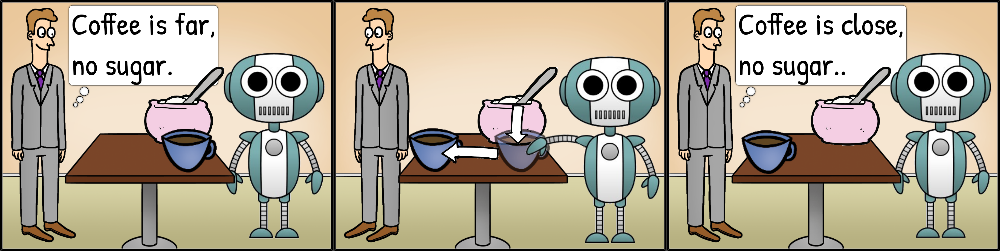
\includegraphics[width=1.0\linewidth]{figures/cartoon_inf_obs_bigger.png}
    \caption{
    % The robot adds sugar to the cup before pushing it while the human is not mindful. The position of the cup is \textit{observable}, so the human can update their belief after observing it. However, since sugar-in-cup is only \textit{inferrable}, and the human was not attentive (\textit{i.e.}, not ``co-present''), the human cannot tell whether sugar is added in the cup.
    % While  
    Human is not attentive when Robot adds sugar to the cup before pushing it forward. \textit{Assessing} the new situation after the two actions, Human can only ``know'' the cup's new position (\textit{observable}), but not \textit{SugarInCup} (\textit{inferrable}).
    }
    \label{fig:obs_attr}
\end{figure}


To better understand these observability classes, consider a scenario with a cup of coffee and some sugar on the table as depicted in Figure~\ref{fig:obs_attr}. 
Initially, the cup is far from the human and without sugar. While the human is not attentive to the scenario, the robot adds some sugar to the cup and pushes it towards the human. 
% Once the human assesses this situation, being attentive 
Once the human is attentive again, they
can notice that the cup is closer. We can say that the position of the cup is \textit{observable}.
However, without observing the robot adding sugar, the human cannot know if some sugar is added to the cup. Hence, we say the \textit{sugar-in-cup} attribute is \textit{inferrable}, 
and the human agent would know if they observed the robot act.
% and the human agent can know when they observe the robot acting.

% For example, suppose after the robot \textit{switches-on} the furnace, the furnace turns {\sc on}, and it is an \textit{observable} fact. So, if the human agent visits the kitchen in the future, they can see that the furnace is {\sc on}.     
% After this switch-on action, suppose next the robot \textit{adds} some salt in the pasta. 
% Naturally, \textit{salt-in-pasta} needs to be inferred (or ``communicated'') as the human cannot directly observe this fact the way the furnace's status was observed. 
% However, such inference only happens when the human agent observes the robot \textit{adding salt} to the pasta. That also means that both agents must be co-present in the kitchen throughout this execution process; otherwise, the human will miss the \textit{salt-in-pasta} fact.  


% A more formal take on usages of these concepts appears in the following section.
% A more formal take on the usage of these important concepts for updating agents' individual beliefs appears in the following section.   

% and $\mathit{un} \in \mathit{Places}$.
% Currently,  are being handled manually,

% such that $\textit{boolVal} \in \{\textit{true},\textit{false}\}$ and only for the constant $kitchen$ it takes \textit{true} for all other object variable from \textit{Places}, the state variable function returns \textit{false}. We note that our current planning system is unable to do this type of reasoning, and hence we take a liberty here to manage it manually so that the main contribution can be targeted. 
% Similarly, action schema is managed as state attributes are also a part of precondition and effect of an action. 

% \begin{definition}
% \textbf{NEW (Location function.)}
% Each \textit{state-variable symbol} is associated to a place through a location function $loc(f_{\textit{svs}}, s) \rightarrow \place \in \places$.
% \end{definition}
% These relations help to describe the world state by expressing where the state-variables are effective and observable. Currently, the locations has to be updated manually in the action's effects.



% Explanation $\observable$ and $\inferrable$.

% \begin{definition}
% \textbf{(Action Observability Function.)}
% \end{definition}



\section{Belief Updating}
% For each agent, there are four ways its belief about the environment can be updated. They are described as follows:
An agent's belief can get updated in four ways as follows: 

\subsection{When It Acts}
% This is the simplest case out of the four. When the agent executes an action its belief is updated based on the action's effect. The current state attributes appearing in the action's effect will be updated with the new values as per this action, while the remaining attributes keep their same old values.
The simplest case. If the agent executes an action, its belief is updated based on its effects. The state attributes appearing in the action's effect get updated with the new values, while the remaining attributes keep their same old values.
% Formally, if the current real state is $s_1$, and the agent (e.g., the robot) executes $a_1$ and generates a new state $s_2$, then the updated belief state is,
% $B_{\varphi_r}^{s_2} = B_{\varphi_r}^{s_1}$ + replaced by the new assignment to the... (we need to introduce many more notations to do it this way) 

\subsection{It Being an Observant}
% Let us first define action observability.

\subsubsection{Action Observability.}
% An action being executed by an agent is \textit{observed} by all other agents co-present with the former, throughout the execution of this action.
% % execution. 
% Therefore, we state that if an agent observes an action being executed, 
% % (and co-present throughout with the acing agent), with the help of situation assessment, 
% the agent infers each \textit{inferrable} effect associated with this action.
An action executed by an agent is \textit{observed} by another agent \emph{co-present} throughout the action execution. Therefore, we state that if an agent observes an action getting executed, the agent will infer the \textit{inferrable} effects of the action.
% or the inferrable state attributes associated to this action.
% i.e., 
Consequently, the agent immediately updates its belief state while each \textit{inferrable} attribute affected by the action receives a new value.  
% with the new value for each state-attribute  affected inferrable} state attribute.

% If the agent 
% is \textit{co-present} with another agent and 
% {\em observes} another agent executing an action throughout,
% If this is the case, 
% then the agent will immediately update its belief with all the \textit{inferrable} effects associated with this action post its execution. 

% In this context, we assume that the robot does not need to be co-present with the human to assess the inferrable and (or) observable effects of the human actions. Moreover, we keep it simple and consider that, in such cases, humans have deterministic decisions to make. Therefore, the robot's belief will always update with the effects of human actions. More complex cases are a part of future work where the robot's belief can diverge from the ground reality, too. 

However, when the human executes an action not observable by the robot, we keep it simple and consider that humans make only deterministic moves. The robot does not need to be co-present to get the effects of human actions. And, its belief state is always updated with both their \textit{inferrable} and \textit{observable} effects. More complex cases are part of our future work where the robot's beliefs can diverge, too. 
% However, when the human executes an action while not being observable by the robot, we keep it simple, considering that humans make only deterministic decisions. 
% Therefore, the robot does not need to be co-present to get the effect of human actions. Also, the robot's belief is always updated with both \textit{inferrable} and \textit{observable} effects. More complex and interesting cases are part of our future work where the robot's belief may diverge from the ground reality. 

\subsection{Via Situation Assessment}

% This work abstractly employs in planning the main ideas of situation assessment based on spatial reasoning and observability.  (we said it!)
The agent assesses the situation from its current location 
with the help of spatial reasoning and its reference frame, i.e., the formal \textit{observability} model. Consequently, the agent updates its existing belief with the relevant ground truth. 
% Note that this also enables the agent to learn an \textit{observable} attribute's value achieved by another agent previously while now the agent shares its \textit{place} with the attribute (Definition~\ref{def:pssav}). 

(Based on Definition~\ref{def:pssav}) We can always associate specific state attributes to \textit{places}. 
For example, suppose that being in the state $s_1$, the robot switches on the furnace placed in \textit{kitchen}, and this generates a new state $s_2$. Also, assume that
% , $\forall s_i \in \mathcal{S}$, $f_{\textit{TurnOn}}^{s_i} 
$f_{\textit{TurnOn}}
% \text{ s.t.  } s_i \in \mathcal{S}
$ is $\observable$ (Definition~\ref{def:svof}).   
% Then, 
% following Definition~\ref{def:pssav}, 
% the \textit{status} of the furnace (\textit{kitch-fur-status}), i.e. 
Then, the \text{place specific attribute function}, $f_{loc} : (...)$, w.r.t. the states
$s_1$ and 
$s_2$ can be expressed as, 
% $f_{\textit{kit-fur-status}} (f_{\textit{TurnOn}} (\textit{furnace}, s_1))$ maps to  $kitchen$, or
$f_{\textit{loc}} (f_{\textit{TurnOn}}^{s_1} )$ and $f_{\textit{loc}} (f_{\textit{TurnOn}}^{s_2} )$, respectively, and both map to $\textit{kitchen} \in Places$.
% such that $kitchen \in \mathit{Places}$.
% or 
% $f_{\textit{kit-fur-status}} (f_{\textit{TurnOn}}: (\textit{furnace}, s_1) \rightarrow \textit{true})$ maps to $\mathit{un}$ such that $kitchen, \mathit{un} \in \mathit{Places}$. 
% Relevant place updates for some specific state attributes, e.g., an action that changes the place of a state attribute like the robot \textit{holding} a cup and \textit{moving} to an adjacent room, are manually handled to make the planning process sound.

Consider the following scenario: The search progresses from $s_2$, along $s_1, s_2, ...$, such that the next action applicable in it is, the agent $(\varphi_h)$ \textit{moving} to the kitchen. This generates a new state $s_3$, and hence $f_{\textit{loc}} (f_{\textit{AgtAt}}(\varphi_h, s_3) )$ maps to $kitchen$, but so does  $f_{\textit{loc}} (f_{\textit{TurnOn}}^{s_3})$. 
% maps to $kitchen$, too. 
In such cases, $\varphi_h$ assesses the \textit{status} of the furnace, i.e., the exact value of $f_{\textit{TurnOn}}^{s_3}$ in $s_3$, which is {\sc on}, and hence the human agent updates their belief.  


% The motivation behind associating each state-attribute of a state to a place is to \textit{define} observability conventions, appearing explicitly in the domain model. 
% % In the current context, 
% A state-attribute (in a state) is classified as either \textit{observable} ($\observable$) or \textit{inferrable} ($\inferrable$). 
% To ``learn'' the \textit{value} of an attribute: 
% % (w.r.t. a state), 
% Either the agent needs to be at the place associated with the attribute such that this attribute is observable and the agent performs situation assessment (described next). 
% Or, if the agent is co-present with another agent who is \textit{acting} and \textit{achieving} the current status (\textit{i.e.}, the effect of the action being executed), while with the help of our situation assessment procedure the agent infers this fact (that is inferrable, of course).
% Or, the agent is communicated about the exact value of this attribute explicitly. Note that attributes belonging to both these classes can be communicated explicitly. 

%%%old relevant text above 

% 
% Which is done using our situation assessment technique (described next). E.g., the human visits $s_2$ and assesses/observes that the furnace is {\sc{on}}. And, to infer a state variable, the agent needs to be \textit{co-present} with another agent who achieves that attribute. E.g., the human needs to be in the kitchen when the robot adds some salt to the pasta, to infer that there is salt in it. 
% 
% To discuss it more formally:

% \textcolor{red}{(FORMAL expression needed? or not? - based on Def~\ref{def:pssav})}

Note that the robot is always aware of the ground reality hence, technically, the idea 
% of situation assessment 
is effective only for the human agent. Here, the robot takes the human's perspective and performs spatial reasoning as per the human's frame of reference or their current location in the environment. 
The human's belief is updated w.r.t. what they can see as ground truth (mimicked by the robot).
This enables $\varphi_h$ to learn an \textit{observable} attribute's value achieved earlier by the robot.
% while currently the human shares their location with the attribute (refer to Definition~\ref{def:pssav}). 
% 
% It predicts the situation and update the belief maintained for the human.
% assessment a collaborative human agent 
% in order 
% to have a better estimate 
% more accurate estimation 
% of their knowledge, and hence of their next possible actions, and thus, to produce better plans.
% This work 
% abstractly employs in planning the main ideas of situation assessment based on spatial reasoning. 
% At planning time, now the robot keeps itself in human's shoes to predict human's belief and emulates their behavior. 
% In this work, we use an existing technology in HATP/EHDA to access the environment, such that the robot keeps itself in human's shoes to predict and emulate human's knowledge and behavior. 
% In this context, the robot's belief is assumed to be the ground truth. However, the human's perspective and belief about the world may be different in different situations. 
% Moreover, it is possible that some object is hidden for the human agent but is visible for the robot even if the agents are together. 
% Thanks to spatial reasoning, one can now define and plan with execution time observability conventions in a principled way. 
% We keep an account on agents' belief divergence that can occur in practice due to spatial reasoning and perspective taking. 

The agent updates its belief with relevant ground truth learned via situation assessment, performed ``immediately'' after the execution of each action. So, technically, the robot performs situation assessment for the human and itself.

\subsection{When It is Being Communicated}
Its belief gets updated by learning ground truth when another agent communicates an attribute-value pair. Communication occurs via a \textit{distinct set} of actions, modeled as a predefined communication protocol for a pair of sender-receiver agents. 
% and they are specified explicitly in the agents' joint task model -- $\mathrm{HTN_r}$ and $\mathrm{HTN_h}$.

As the robot is always aware of ground truth, technically, it is effective only for human beliefs.
The human receives an attribute and its exact value at the current stage from the robot, and, accordingly, their belief gets updated. 
We note that each action communicates only {\em one} attribute-value pair, so just one attribute gets updated in the human belief.

% In the next section
% it needs to make decision "if", "when", and "what" to communicate with these explicit actions.

\section{Planning With Communication Actions}
% As human's belief can diverge from the ground-truth, the robot need
For an agent to decide ``if'', ``when'' and ``what'' to \textit{communicate} to another agent, it first needs to establish a common protocol with that agent even before planning.  
In this work, we establish such communication protocols between each sender-receiver agents pair, where we use speech modality, and model explicit communication actions between two agents. 
% They appear in their joint task model, 
However, we note that these actions are different than agents' (non-) primitive actions, and they are used only in special circumstances during planning.

\subsection{Modeling Communication Actions} 
We give a generic communication action model in this context. 
% which will later be used for the case, when the robot is aware of the ground truth, while the human's belief diverges from the real world.
% 
Suppose there exists a state-variable function, $f_{svs}:(?g_1 (gr_1), ?g_2 (gr_2), ..., ?g_k (gr_k),\mathcal{S}) \rightarrow ?g_{k+1} (gr_{k+1})$ such that,
% $f_{svs_i}^s$, 
% Such that, 
for the current world state $s \in \mathcal{S}$, the corresponding state attribute, $f_{\textit{svs}}(g_{(1)l},g_{(2)m},...,g_{(k)n},s)$ maps to $q$.

An agent $\varphi_i$ can \textit{communicate} this attribute-value pair to another agent $\varphi_j$, if the following conditions meet as action precondition: 
(1) For $\varphi_i$, its belief state satisfies the fact being communicated, i.e.,
$f_{\textit{svs}}(g_{(1)l},g_{(2)m},...,g_{(k)n},B_{\varphi_i}^s) = q$, and (2) $\varphi_j$'s belief state does not satisfy this truth, i.e., $f_{\textit{svs}}(g_{(1)l},g_{(2)m},...,g_{(k)n},B_{\varphi_j}^s) = r$ such that $r \neq q$.
The effect of this action is that now 
% the attribute gets the true value and 
$\varphi_j$'s belief is updated, i.e., $f_{\textit{svs}}(g_{(1)l},g_{(2)m},...,g_{(k)n},B_{\varphi_j}^s) \leftarrow q$. 
% That means, the attribute receives the correct value and belief is
% is assigned 
% the \textit{exact} value, i.e., 
% $q$.

% 
% $f_{svs_i}^{B_{\varphi_i}^s} \rightarrow q$. And, for $\varphi_j$, its belief state diverges on this fact, i.e., $f_{svs_i}^{B_{\varphi_j}^s} \rightarrow r \text{ and } q \neq r$. 
% (2) 


% \textcolor{red}{to be continued ******}

\subsection{Planning with Reasoning on Human Mental State }
Now that we have defined and described all essential tools, we describe the new approach and explain how these tools are utilized by it. 
First, we note that we put an effort to make our main contributions to have a ``generic'' description. Hence, they are not limited to only our intended HATP/EHDA architecture, which we plan to enhance in this paper.
% in this work.

% The solver is based on the HATP/EHDA framework that is the underlying planner~\cite{buisan:hal-03684211}. 
% However, 
We only describe the \textit{main changes} made to enhance the underlying solver. 
Suppose an agent applies an action: First, the belief states of all agents co-present with this agent get updated with the action's inferrable effect. Later, the \textit{situation assessment} process is used for every other agent to assess the changes (captured via observable state attributes). As a result, their beliefs are updated by the observable effects if the required conditions are satisfied. We discussed these subroutines in detail in earlier sections.

\begin{figure*}[!ht]
    \centering
    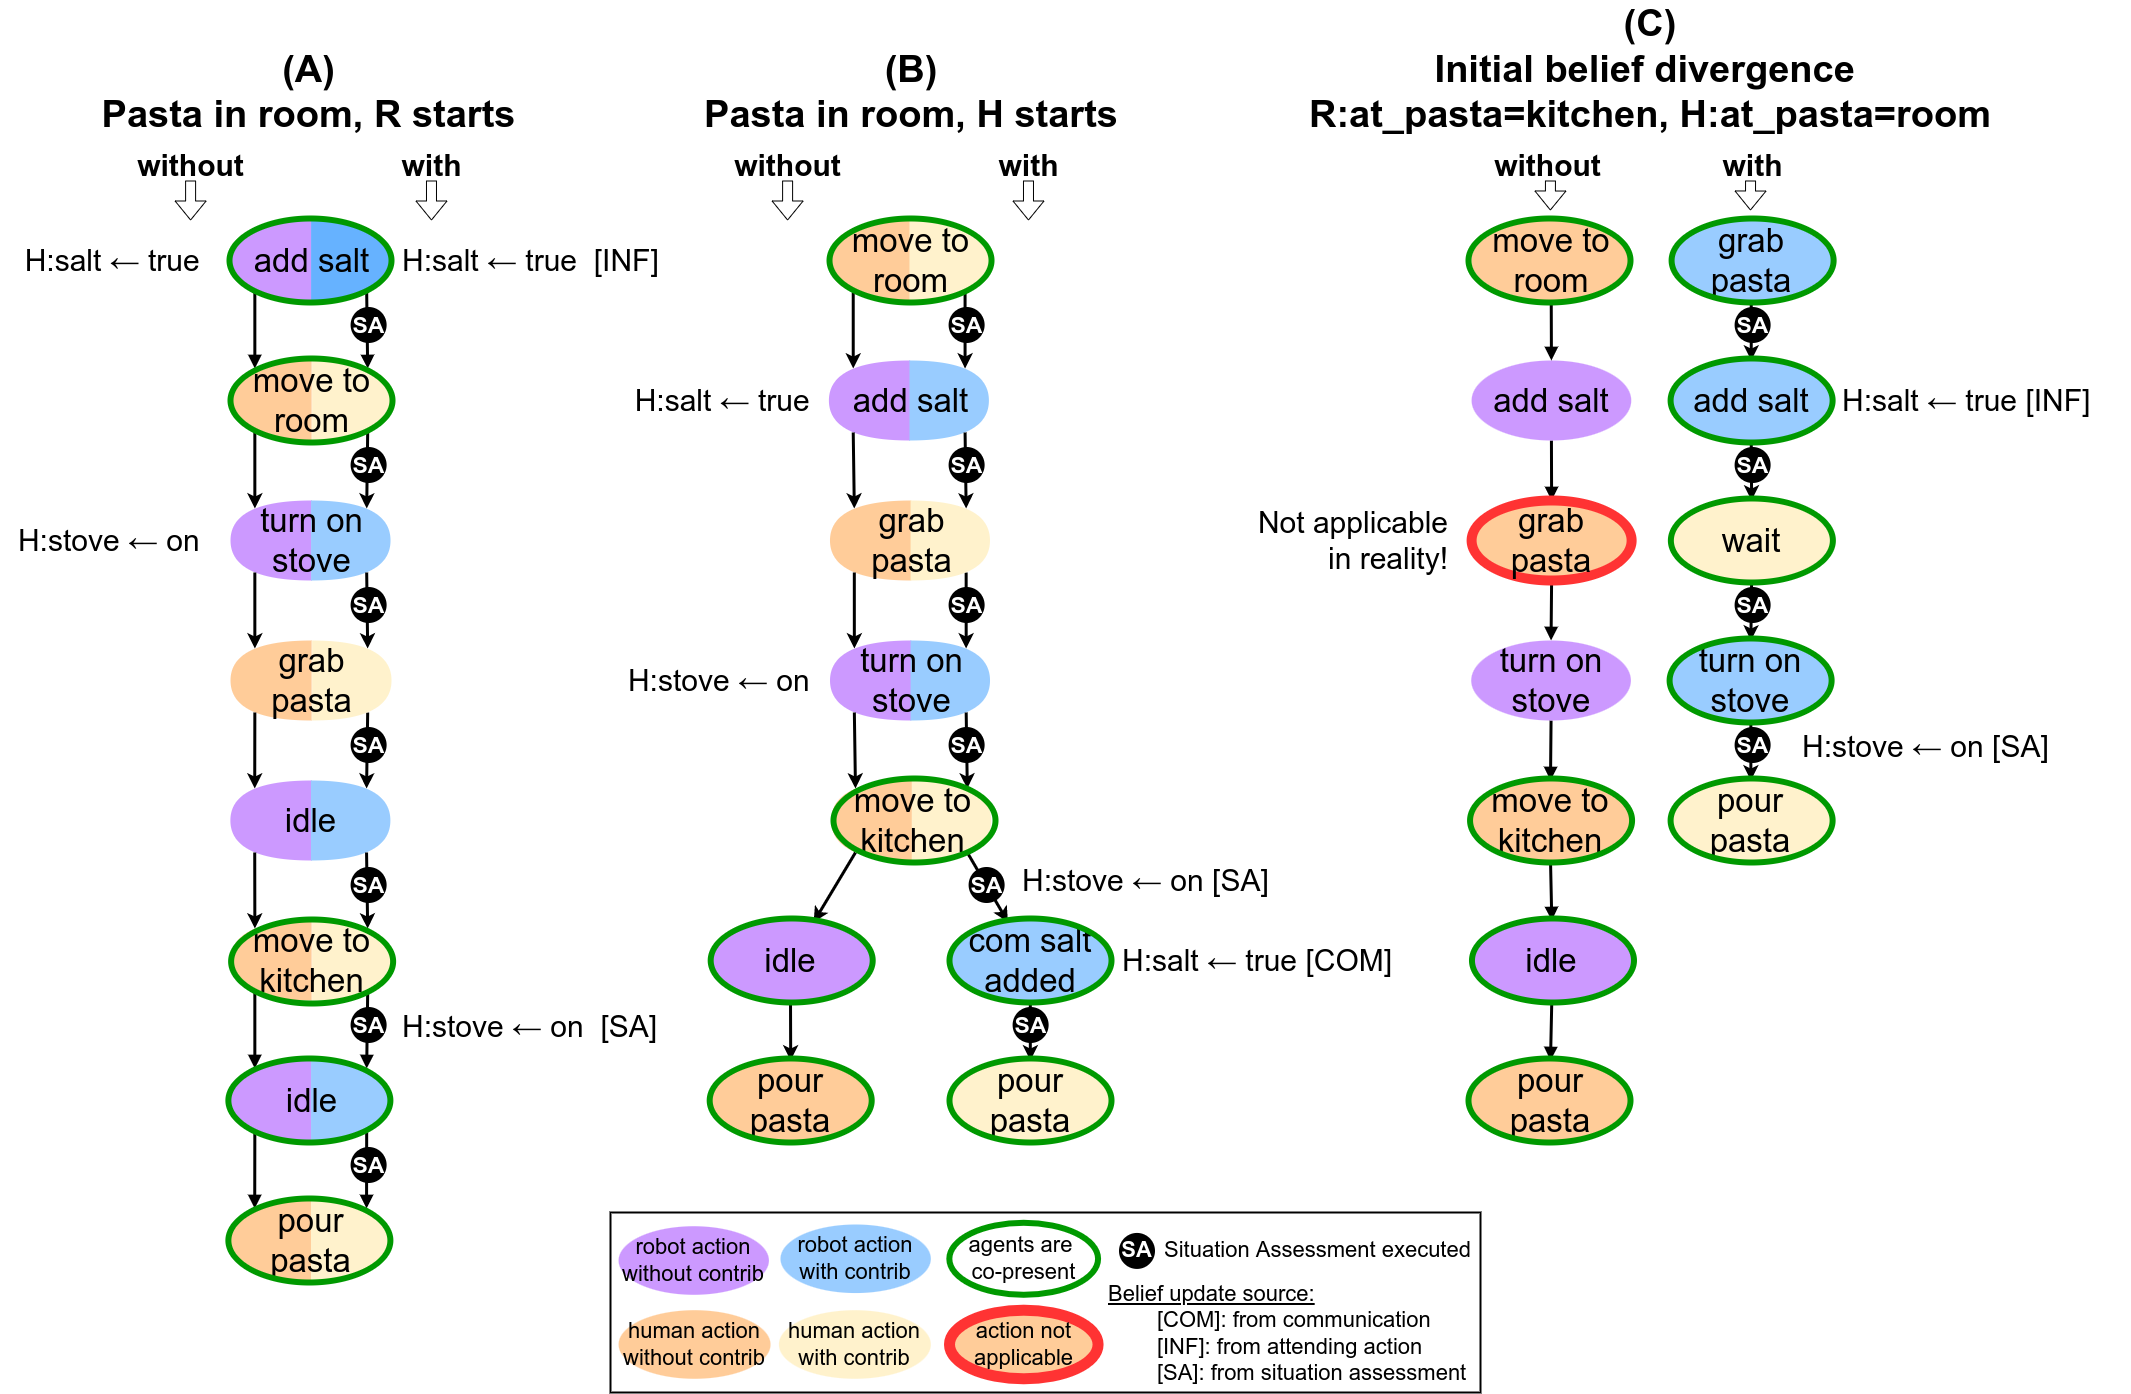
\includegraphics[width=0.85\linewidth]{figures/example_cook.png}
    \caption{
    Shows the plans obtained in three scenarios: Each scenario presents two plans --- on the left, obtained by the old solver, and on the right, obtained via the proposed solver. The latter depicts more realistic and appropriate belief updates (as proposed to be tackled).
    Case~(A): the plans are the same, but the updates in the human belief are more realistic with our approach. Case~(B): the human has no certainty on {\em SaltInPot}, while ours decides to communicate to remove the ambiguity. And, Case~(C): the initial belief divergence induces an ``invalid'' plan, but our approach predicts that the human agent will \textit{assess the situation} and update their belief with all the facts without being communicated. (Other minor details are outlined in the figure.)
    }
    \label{fig:scenarios}
\end{figure*}

\subsubsection{Communication in Planning}
% There are two new phases in our algorithm 
% that differs from the underlying planner's algorithm, 
The following essential changes in the existing algorithm support efficient communication in planning. 
(Recall the sender-receiver pair discussed earlier.) The approach identifies whether the receiver's belief divergence is \textit{relevant}, and thus if the receiver's belief needs to be corrected.
% Second, to identify all state attributes w.r.t. the ground truth where the receiver agent's belief differs, and to decide which all must be communicated (to communicate minimally and avoid verbosity), to make sure that the remaining divergences in the updated receiver's belief are \textit{not} effective. 
If so, all state attributes where the receiver agent's belief differs w.r.t. the ground truth are identified. Then, we decide which of these state attributes and their exact values must be transmitted by the sender (\textit{i.e.}, the robot), supporting the idea of communicating minimally and avoiding verbosity. Once we determine that, the receiver's (\textit{i.e.}, human's) belief gets updated accordingly, ensuring that the remaining false knowledge of the receiver's updated belief is \textit{not effective}, which also means that the belief divergence is not relevant anymore. 
    

% \subsection{Relevant Belief Divergence}
% \subsection{Collect All the Belief Divergences}

% \begin{figure}
%     \centering
%     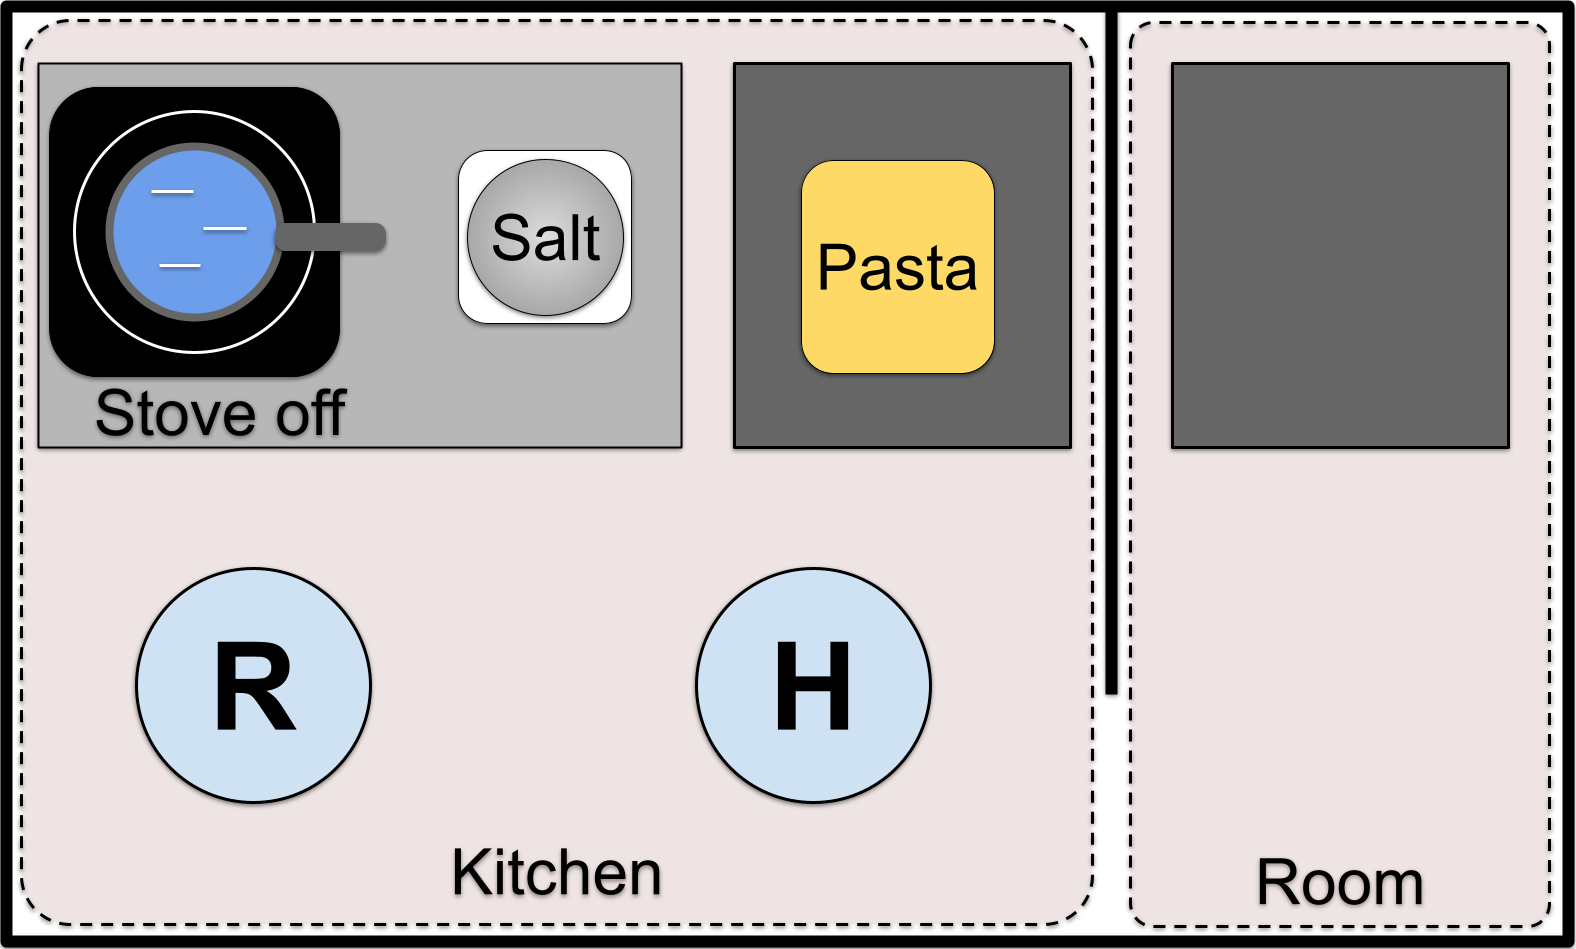
\includegraphics[width=0.7\linewidth]{figures/scene.png}
%     \caption{The cooking pasta domain.}
%     \label{fig:scene}
% \end{figure}

\begin{itemize}
    \item \textbf{Relevant Belief Divergence.}
    At a given stage, if the human agent, based on their own belief, can perform a set of actions that differs from 
    the one 
    the human could perform w.r.t. to the robot's belief (or the ground reality), then we say that such divergence in their belief is \textit{relevant}.
    % 
    A divergence is also declared as \textit{relevant} if an action has different effects w.r.t the other agent's belief.
    However, currently, our reasoning system is myopic: We do not evaluate in a principled way the impact of \textit{different} actions that humans could execute (based on their wrong belief), or of \textit{different} effects, with their overall positive and detrimental effects on achieving the joint task. At this stage, it simply ``decides'' to align the agent's beliefs using communication actions whenever the belief divergence is relevant.
    However, a smarter approach would probably be to analyze the history of plan trace(s) or agents' future actions to decide whether their beliefs should get aligned or not, or for that matter, how much to communicate, but it is currently out of the scope of this work. 
    % This we intend to tackle in future.
    % .  
    % But, for now, 
    
    \item \textbf{Communicate Only The Required Facts.}
    % Now that we decided to align the human's belief with the ground reality, 
    It ``decide'' the \textit{essential} changes in the human's belief at this stage to be made such that the relevance of their updated belief (which could still be diverging) becomes ineffective. 
    (In the worst case, the robot communicates all the divergent attribute-value pairs, and their belief states are perfectly aligned.) The subroutine used to decide which all communication actions will appear in the robot's executable plan; is described in the following steps:
    \begin{enumerate}
        \item 
        % Store all the state attributes and their values such that
        \textit{Store} each attribute and its value if the attribute's value differs in the human's belief from the robot's belief. 
        % these variables' values differ in the human's belief as compared to the ground reality. 
        % I.e. $$
        \item For each stored attribute-value pair, \textit{build} a communication action, $\textit{comm-action}_i$, based on the model described earlier. They are considered equally costly.  
        \item 
        % From the current stage of planning, say from the state $s_i$, follow the Breadth-First Search (BFS) ordering. 
        At a given stage (of planning), e.g., the ground truth $s_i$, follow the Breadth-First Search ordering. 
        The \textit{source} is $B_{\varphi_h}^{s_i}$, and each $\textit{comm-action}_i$ changes and aligns \textit{exactly} one attribute while its updated value satisfies the ground truth. If $\textit{comm-action}_i$ is applied, generates a new belief state (following the regular state transition rules), using: $B_{\varphi_h}^{s_i,1} = \gamma(B_{\varphi_h}^{s_i}, \textit{comm-action}_i)$.
        % The source is $B_{\varphi_h}^{s_i}$, such that each $\textit{comm-action}_i$ changes and aligns \textit{exactly} one state attribute such that its updated value satisfies the ground truth. 
        % The applicability of $\textit{comm-action}_i$  generates a new belief state, following the standard state transition rules in classical planning, i.e., 
        % $B_{\varphi_h}^{s_i,1} = \gamma(B_{\varphi_h}^{s_i}, \textit{comm-action}_i)$. 
        It \textit{continues} until the very first (updated) human belief is \textit{chosen} to expand while the remaining belief divergence in it is ineffective. 
        We then \textit{retrieve} all the actions used from the root until the current belief state.   
    \end{enumerate}
    
    % \textcolor{red}{*** to be continued ***}
\end{itemize}


Following our approach, the robot uses the required communication actions after each stage of plan elaboration, i.e., HATP/EHDA's plan elaboration. 
It then uses the predefined communication modality to interact with the human agent during execution via these communication actions. 

% \section{Soundness and Completeness***}

% \textcolor{red}{\textbf{unpolished text below (START)}}

% Important section for "planning" conference like aaai, icaps. Less important for HRI related conf
% \section{Theoretical Properties}
% \begin{theorem}
% \textbf{(Soundness.)} The new planning algorithm is sound if the underlying planner is sound.
% \label{planner:soundness}
% \end{theorem}
% \begin{proof}
% TODO
% \end{proof}

% \begin{theorem}
% \textbf{(Completeness.)} The new planning algorithm is complete if the underlying planner is complete.
% \label{planner:completeness}
% \end{theorem}
% \begin{proof}
% TODO
% \end{proof}


% \section{Empirical Evaluation}

% TODO


% 

% % what is known ? our understanding of the world
% General context, towards robot partner. 

% % what is unknown ? the gap we want to fill
% % how and why ? your rational and purpose/hypothesis 

% \textbf{Choice to reduce ambiguities [example, as introduction]}:
% Let's assume the human and the robot have to cook together and at some point salt needs to be added to a dish. The robot adds salt to the dish while the human is away. When coming back, the human has no way to know if there is salt just by looking at the dish.
% Then three cases can occur : 1) The human considers that the robot didn't add salt, thus they will to add more, 2) The human considers that the robot added salt, so the goal is reached, 3) the human prefers to directly ask the robot if it added salt. 
% Humans are rational, so they will rarely blindly act without at least asking the state of the shared plan. However, whatever case we are in, an ambiguity will remain for the human, and we are able to predict it. Thus, we decide to proactively reduce the ambiguity by communicating about their belief divergences or the missed actions. This communication might seem optional in some situations but having a plan without ambiguities in the context of a shared goal is often much better than a plan with fewer steps but where agent aren't sure about what they have to do.

% \section{Background}
% HATPEHDA concept and definitions

% The work \cite{buisan:hal-03684211} already support collaborative task planning while maintaining distinct beliefs/knowledge for each agent. This work is itself an extension of HATP \cite{hatp?} having one search thread for a shared plan resulting in two coordinated plan streams. The last work HATPEHDA proposes a two threads search. Based on this work, we enhanced the task planner with a few concept linked to perspective taking and observability in order to reduce the ambiguities that may happen in a collaborative task. First we predict the situation assessment of an agent. On the other hand, we look for belief divergences that have a detrimental influence on the plan in order to fix them with communication. We also check observability of action execution to update beliefs with different types of effects.

% Agents can have a shared goal but no shared plan. There is no plan negotiation between the agents, so the robot is only able to estimate what the human will do and plan its own actions according to that.

% \subsection{HATPEHDA background/basis and definitions}

% The main structure manipulated by our planner is the \textbf{agent}, more precisely two will be represented, the \textit{human} and the \textit{robot}. Each agent has their own \textbf{beliefs}, \textbf{action model}, \textbf{agenda}, \textbf{plan} and \textbf{triggers}. The planner has to use their action models and beliefs to decompose the tasks in their agenda into primitive tasks (actions) that are inserted in their plan. By doing so, it also has to update the beliefs of each agent and to model their reaction by executing the triggers. \cite{buisan:hal-03684211}.

% The agents, robot and human, have each a distinct action model modeled with HTNs. The robot HTN starts with the goal given to the robot and describes how to decompose that abstract goal into several actions. The human HTN represents the anticipation by the robot of the human plan and possible actions in a given situation. Other formalism like POMDP or PDDL could be used to describe the agents' action models as soon as they provide the next possible actions of an agent in a given state. Especially the human one which is an estimation.

% The planner has a goal creation mechanism, especially for the human, based on goal-directed or situation-directed task creation.

% The planning algorithm is implemented as a search involving two threads: 1) the robot task-based plan search using the robot action model 2) the estimation of the human task-based plan search using the human action model.

% While HTN-R corresponds to the controllable part  (from the robot point of view) of the (shared) plan, HTN-H represents the contingent part of the plan: the decisions and actions of the human. 

% Hence, the obtained plan has two streams (one for the human and one of the robot) and is conditional. Alternatives correspond to human decision: choosing to act or not, making one (out of several choices).

% As a result, HATP/EHDA allows to clearly separate what is planned for the robot and what the human can potentially do with respect to the task at hand. Besides, it allows to also:
% \begin{itemize}
%     \item deal with cases where the task is only given to the robot and not shared by the human
%     \item manage the creation of a shared goal
%     \item provide a mean to implement elicitation, by the robot, of decisions or reactions of the human
% \end{itemize}
% In our case the plan process starts:
% \begin{itemize}
%   \item with a goal given only to the robot: a task placed at the root of HTN-R (ex: Human asks the robot to achieve a goal)
%   \item or with a shared goal: the same task is placed at the roots of  the two HTNs (ex: Human says to the robot: "Let us do X")
% \end{itemize}

% Situation-directed task creation in HTN-H allows to model (potential) reaction by the human to a situation created by after a given action of the robot. This can be used in the planner to elicit a reactiion of the human.

% \textbf{HTN formalism [in background ?]}:
% An HTN \textit{planning problem} is the 3-tuple $\langle d, S_0, \mathcal{D} \rangle$, where $d$ is the sequence of (primitive or abstract) tasks to solve, $S_0$ is an initial state as in classical planning, and $\mathcal{D}$ is an HTN \textit{planning domain}. Specifically, an HTN \textit{planning domain} is the pair $\mathcal{D}=\langle\mathcal{A},\mathcal{M}\rangle$ where $\mathcal{A}$-the primitives of the domain-is a finite set of operators as before, and $\mathcal{M}$ is a finite set of \textit{methods}. A \textit{method} is a tuple consisting of the name of the method, the abstract task that the method is used to solve, a precondition specifying when the method is applicable (like an operator's precondition), and a \textit{body} indicating which tasks are used to solve the task associated with the method. The method-body is a sequence of primitive and/or abstract tasks. 

% The planning process works by selecting applicable reduction methods from $\mathcal{M}$ and applying them to abstract tasks in $d$ in a depth-first manner. In each iteration this will typically result in $d$ becoming a "more primitive" sequence of tasks. The process continues until $d$ has only primitive tasks left. At any stage in the planning process, if no applicable method can be found for an abstract task, the planner essentially "backtracks" and tries an alternative method for an abstract task refine earlier.

% \textbf{Computing next possible agent actions / refining agenda [nothing new here, in hatpehda background ?]}:
% The refinement of the HTNs is mostly done thanks to the function $refineAgenda()$. This function keeps refining the agenda of an agent in a given state until reaching a not done primitive task at the first spot. It returns a refinement which is list of decomposition, one for each applicable methods. Each decomposition is a list of the obtained subtasks which starts with a not done primitive task. The second parameter the function $refineAgenda$ can be used to specify with which beliefs the refinement has to be done. 
% The action model of each agent is described with a HTN. Thus, the process to compute (or estimate in the human case) the next possible actions of an agent is very close to classic HTN refinement.
% The classic planning process for HTN planning problem consist in selecting applicable reduction methods from $\mathcal{M}$ and applying them to abstract tasks in $d$ in a depth-first manner. In our contribution the planning process slightly differs from the classic process since the goal is to compute or estimate all possible next actions in a given state. 
% Here, $d$ corresponds to what we call the agenda of the agent. To compute the next possible actions the agent's agenda is refined. To do so the first task in the agenda is popped, and all applicable reduction methods are applied to the task resulting is search branches with different subtasks. The process is repeated for each created branch until reaching a primitive task in each of them. The primitive tasks from each search branch constitute the set of all possible next actions of the agent.
% A search branch can refine into nothing but if all search branches refine into nothing then the first task popped from the agenda is done, so the next task in the agent's agenda is popped and refined. 
% A search branch, corresponding to a list of subtasks, is called a decomposition. The list of all obtained decompositions is called a refinement.  


% \section{Materials and Methods}
% % what did you do ?



% \subsection{Knowledge representation and observability definitions}

% Our formalism is close to the SAS+ Formalism applied to HTN.(Probably to remove, might bring more confusions than explanations)

% \textbf{Word state}: 
% Let $\worldstates$ be the set of all possible world states. World states are defined by a same set of fluents. Each world state is fully described by the value of all its fluents at a given time i.e. $\forall\worldstate\in\worldstates, \worldstate=\{ \fluent{\worldstate}{}{} \}$.

% \textbf{Fluent}: 
% A fluent $\fluent{\worldstate}{}{}$ is a multi-valued state variable associated to a finite domain $\dom{\fluent{\worldstate}{}{}}$ partially describing the state of the world at a given time.

% % (introduce loc ?)
% % The observability type of fluents is qualified through the relation $\obs{ \fluent{\worldstate}{}{} } \in \{ \observable, \inferrable \}$. 

% e.g. Considering the following fluent $\fluent{\worldstate}{}{temp\_water}$, if initially the water is hot then $\fluent{\worldstate_0}{}{temp\_water}=hot$.

% \textbf{Belief divergence}: 
% We note $\fluent{\worldstate}{,\agent}{}$ a fluent evaluated in the perspective of an agent $\agent$. Thus, for a given real state of the world $\worldstate\in\worldstates$, the robot and the human can have different values for the same fluent. We call such mismatch a belief divergence.

% e.g. $(\fluent{\worldstate_0}{,\robot}{temp\_water}{}=hot) \neq (\fluent{\worldstate_0}{,\human}{temp\_water}=cold)$

% \textbf{Two distinct Beliefs}: 
% We call beliefs of an agent $\agent$, noted $\beliefs_\agent$, the belief state in which this agent thinks the world is in, i.e. the set of all fluents evaluated in their perspective at a given time: $\beliefs_\agent=\{ \fluent{\worldstate}{,\agent}{} \}$. It is important to note that we use two distinct belief states during the planning process. On one hand, we consider the beliefs of the robot $\beliefs_\robot$ which are obtained through perception and effects of robot actions and decisions. And as we consider the planner as being part of the robot, we assume that $\beliefs_\robot$ is the ground truth estimation for the planner. On the other hand, we consider the human's belief state $\beliefs_\human$ which is only estimated by the robot by doing some perspective-taking reasoning during the planning process (and before ?).

% \subsection{Place-based observability model}

% We introduce a place-based model of observability. An agent observes and can only observe what happens in their current place, this includes action executions and fluent values.

% \textbf{Places}: 
% A place is an area defined a priori in the environment. Let $\places=\{ \place_i \}$ be the set of all defined places. Agents are always situated in a place or moving between them. Two agents situated in the same place are said to be co-present. Actions are always performed in a place. (Most?) State variables are associated to a place.

% \textbf{Observation of an action execution}: 
% The execution of an action performed by an agent $\agent$ is observed by all agents that were co-present with $\agent$ either before or after the action. The co-presence is checked both before and after to cover navigation actions.

% \textbf{Observability of fluents}:
% Each (most?) fluent is associated to a place $\place \in \places$ through the relation $\loc{ \fluent{\worldstate}{}{} }=\place$. These relations help to describe the world state by expressing where the fluents are effective and observable. (If $\loc{ \fluent{\worldstate}{}{} } = \varnothing $ then the fluent is ubiquitous). These relations can be dynamic for example when the fluent describes a property linked to a moving entity. Currently, the location of a fluent has to be updated manually in the domain if it is dynamic (we should go for an "entity-based" description of the world state to automatically update).

% The observability type of each fluent is constant and defined initially through the relation $\obs{ \fluent{\worldstate}{}{} } \in \{ \observable, \inferrable \}$. 
% The first value $\observable$ means that the fluent is observable. A fluent is observed by an agent only if it is observable and if that agent is in the place associated to the fluent. 
% Note that places can be symbolic and not only physical/geometric to represent more complex situation. For instance, let's consider the fluent $\fluent{\worldstate}{}{at\_o}$ describing the position of an object \textit{o}. The object is in the kitchen inside a cupboard that can either be open or closed. This situation can be modeled as follows :
% \begin{itemize}
%     \item $\fluent{\worldstate}{}{at\_o}=cupboard$
%     \item $\obs{ \fluent{\worldstate}{}{at\_o} }=\observable$
%     \item $\loc{ \fluent{\worldstate}{}{at\_o} } \in \{ kitchen, closed \}$
% \end{itemize}
% The relation $\loc{ \fluent{\worldstate}{}{at\_o} } = kitchen$ corresponds to when the cupboard is open, which means any agent in the place $kitchen$ can observe the object. On the other hand, when the cupboard is closed, $\loc{ \fluent{\worldstate}{}{at\_o} } = closed$, the agent cannot observe the object.

% The other value $\inferrable$ qualifies inferrable fluents. A fluent is inferrable if its value isn't observable but can be inferred by attending an action affecting that fluent. For instance, by observing someone adding salt to a dish we infer that there is now salt in the dish, although the salt in the dish isn't observable. It means that without attending the action execution it's impossible to tell if there salt just by looking at it. Thus, when an action affects inferrable fluents only the co-present agents gets their beliefs updated. We later refer to actions affecting inferrable fluents as actions with inferrable effects (resp. with observable effects).


% \subsection{Beliefs updates}

% Agents' beliefs are updated by four different processes: 1) performing an action, 2) attending inferrable effects, 3) assessing the situation, and 4) communicating about a relevant belief divergence.  

% \textbf{Performing actions / Inferrable effects}: 
% When an agent performs an action its own beliefs are always directly updated with the action's effects.

% The other agent's beliefs are updated about these effects through two mechanisms. The first one, that will handle observable effects, is the situation assessment and is detailed just after. 
% The second one concerns inferrable effects. As mentioned before, only agents that observed the action execution get their beliefs updated with the inferrable effects.

% For now, we assume that if we estimate that the human will perform a task not observable by the robot then it should remain quite simple like a series of deterministic actions. Basically, we currently do not handle more complex cases where the human has multiple choices of actions while not being observable. Considering this hypothesis, the robot beliefs are always updated with the effects of human actions, weither they are co-present or not.

% \textbf{Situation Assessment}:
% The idea is to predict the situation assessment of an agent and update their beliefs according to what they can see in their current place. When executed, each agent $\agent$ updates their beliefs with the ground truth value of every observed fluents, i.e. for every observable fluents ($\obs{ \fluent{\worldstate}{}{} } = \observable$) located in their place ($\loc{\fluent{\worldstate}{}{}} = \fluent{\worldstate}{}{at\_\agent}$), we have $\fluent{\worldstate}{,\agent}{} \gets \fluent{\worldstate}{}{}$. The situation assessment is executed after every action execution. This way, the agent's beliefs are updated either with the observable effects of an action performed by another co-present agent, or with the observable effects they missed when entering another place. 
% Note that since the ground truth is actually the robot beliefs, this situation assessment is only effective for other agents, so here the human. 

% \textbf{Relevant belief divergences checking}:
% We want to detect if a belief divergence influences the plan of the human, i.e. if when using the human beliefs containing belief divergences induces different human actions than the ones expected using the ground truth beliefs. If so, the belief divergences are qualified as relevant. Indeed, a belief divergence can wrongly affect the applicability of a human action, its cost and its effects. 
% Any difference in the human plan makes it either not applicable in reality, more expensive or with undesired effects. There are some rare cases of belief divergences inducing a different plan still applicable, with a similar cost and no undesired effects. But for now we omit those cases, and we consider relevant belief divergences as always detrimental. 
% Note that there can be belief divergences not affecting the plan which will not be considered as detrimental.

% To check if there are some relevant belief divergences we proceed as follows. When refining the human agenda to estimate their next possible actions, we first use the human beliefs $\beliefs_H$. The process is repeated but considering the robot beliefs $\beliefs_R$ (ground truth). The two obtained refinements are then compared to check if they are the same. Two refinements are considered to be the same if they respectively have the same decompositions, i.e. if, in both refinements, each decomposition respectively has the same type, subtasks and if their actions have the same applicability, cost and effects. 
% If a difference is spotted we consider that there are relevant belief divergences to align, but we don't know which ones yet.

% \textbf{Identify the relevant divergences and communicate}: 
% Once the presence of relevant belief divergences has been confirmed they have to be identified. All divergences between $\mathcal{B}_R$ and $\mathcal{B}_H$ are first computed. Then the divergence's corrections are simulated one after another (i.e. $ \fluent{\worldstate}{,\human}{i} \gets \fluent{\worldstate}{,\robot}{i}$) and the human agenda is refined again in order to compare the new refinement with the one previously obtained with $\beliefs_\robot$. We keep simulating combination of divergence corrections in a breadth-first (search) manner until the refinements are the same, which means that all the relevant divergences have been identified. In the worst case, the two refinement are not the same until reaching the last combination which corresponds to all divergences being corrected, thus where $\beliefs_\human$ and $\beliefs_\robot$ are the same. So the obtained refinements will necessarily be the same which guarantees the ending of our algorithm. After having identified the divergences to correct in order to obtain the same refinements, the corresponding communication action is inserted in the robot's plan to inform the human about their relevant belief divergences and to correct them.
    
% Communication actions are supposed to be instantaneous and able to correct several divergences at once. For now they are inserted right before the detected erroneous human action. (A more complex reasoning could be added to identify the optimal place to insert the communication action in the plan). 

% \textbf{Choice to reduce ambiguities}:
% In the case of a shared goal, let's assume that the human didn't observe the robot performing an action with only inferrable effects, so when coming back the human has no way to tell if the action has been done just by looking at the scene. 
% Then three cases can occur : 1) The human considers that the robot didn't perform the action, thus the human will try to perform it again, 2) The human considers that the robot performed the action, so the plan execution continues, 3) the human prefers to directly ask the robot if it performed the action. 
% Humans are rational, so they will rarely blindly act without at least asking the state of the shared plan. However, whatever case we are in an ambiguity will remain for the human, and we are able to predict it. Thus, we decide to proactively reduce the ambiguity by communicating about their belief divergences or the missed actions. This communication might seem optional in some situations but having a plan without ambiguities in the context of a shared goal is often much better than a plan with fewer steps but where agent aren't sure about what they have to do. Communication help to compel the human actions.


% \subsection{Algorithm (Optional maybe ...)}
% MAYBE OPTINAL because it involves mechanisms not introduced (or maybe we should introduce them in the background ?) like the triggers and the WAIT/IDLE actions.

% The refinement of the HTNs is mostly done thanks to the function $refineAgenda()$. This function keeps refining the agenda of an agent in a given state until reaching a not done primitive task at the first spot. It returns a refinement which is list of decomposition, one for each applicable methods. Each decomposition is a list of the obtained subtasks which starts with a not done primitive task. The second parameter the function $refineAgenda$ can be used to specify with which beliefs the refinement has to be done. 

% The returned refinement in Alg.~\ref{alg:ap_ref_all} contains the subtasks obtained through the refinement of the agenda after a potential belief alignment, application of the actions, situation assessment and triggers.

% \begin{algorithm}
% \caption{Get applied refinement ALL}\label{alg:ap_ref_all}
% \begin{algorithmic}
% \Require $h\_name$: human name, $r\_name$: robot name, $ags$: all agents

% \State $ref \gets refAgenda(ags, ag\_name)$

% \State $ref\_r \gets refAgenda(ags, r\_name)$ \Comment{H only}
% \If{$relevantDivergences(ref, ref\_r)$} \Comment{H only}
%     \State $alignBeliefsWithComAction()$
%     \State $ref \gets refAgenda(aligned\_ags, h\_name)$
% \EndIf

% \For{$decomp$ in $refinement$}

%     \State $result \gets applyOperator(dec, ag\_name)$ 
%     \If{$notApplicable(result)$}
%         \State \texttt{add wait, idle or end}
%     \Else
%         \State $applyOperator(dec, r\_name)$ \Comment{H only}
%         \State $applyInferrableEff(dec, h\_name)$ \Comment{R only}
%         \State $humanSituationAssessment()$
%         \State $checkTriggers()$
%         \State $updateDecomp(decomp)$
%     \EndIf
% \EndFor

% \State \Return ref

% \end{algorithmic}
% \end{algorithm}

% \textcolor{red}{\textbf{unpolished text (END)}}


% \usepackage{multirow}
\begin{table}
    \begin{adjustbox}{width=0.85\columnwidth,center}
    \begin{tabular}{@{}c|r r r|r r@{}}
        % \hline
        \multirow{2}{*}{
        \textbf{Domain}} & \multicolumn{3}{c|}{\textbf{\textit{Old Solver}}} & \multicolumn{2}{c}{\textbf{\textit{Our Solver}}}
        \\
        % \cline{2-6}
        & \multicolumn{1}{c}{\textit{S}} & \multicolumn{1}{c}{\textit{NA}} & \multicolumn{1}{c|}{\textit{IDL}} & \multicolumn{1}{c}{\textit{S}} & \multicolumn{1}{c}{\textit{Com}} 
        \\ \cline{1-6}
        % \hline
        \textit{Cooking} & 18.6\% & 77.0\% & 23.0\% & 100\% & 54.9\%\\
        % \hline
        \textit{Box} & 25.0\% & 83.3\% & 16.7\% & 100\% & 68.8\%\\
        \hline
        \textbf{Average} & 21.8\% & 80.2\% & 19.9\% & 100\% & 61.9\%\\
        % \hline
    \end{tabular}
    \end{adjustbox}
    \caption
    {
    \label{tab:q_results}
    % Comparison of the two solvers on the two domains. 
    In each domain: for the \textit{old solver}, the success rate (\textit{S}), the ratio of failed plans due to a non-applicable action (\textit{NA}), and the ratio of failed plans due to an inactivity deadlock case (\textit{IDL}), while for \textit{our solver}, the success rate (\textit{S}) and the ratio of plans including a communication action (\textit{Com}).
    }
\end{table}

\section{Empirical Evaluation}
Before we describe the domains used for the experiments and results, first, we make a \textit{high-level} distinction between the existing and new approaches. 
In principle, the existing solver can handle agents' individual belief divergences, but ``not during planning'' unlike our approach. To achieve that, the existing solver can use a cumbersome technique that intervenes by updating the (collaborative) task networks of the joint task model/specifications while using triggers.
% ~\cite{thesisBuisan21}. 
% 
% note that the existing system is not sound as it claims to handle human decision and action or whatever... but in principal, is able to produce unsound plan. This will appear in the theoretical guarantees... not in the main text
% Also, they must divergence must be part of the initial belief. 
% as there in no way robot .     

We consider two domains 
% (described in what follows) 
to compare the two approaches.
% show the applicability and utility of the proposed approach.

% \paragraph{Domain  Description}
% We consider two domains 
% % (described in what follows) 
% to show the applicability and utility of the proposed approach.

\subsubsection{Cooking Pasta Domain:}
% Also, in the running example of the paper, this domain captures a robot and a human cooking pasta collaboratively, presented in Figure~\ref{fig:scene}. Suppose the agents have different roles in achieving the task. The robot \textit{adds} salt to the pot and \textit{turns-on} the stove. The human \textit{grabs} the pasta and \textit{pours} it into the pot. Pasta can be poured only after salt is added, and the stove is {\sc on}.
(It is also the running example.) Suppose a stove and salt are available in \textit{Kitchen} (belongs to $\textit{Places}$), and the pasta can be located either in \textit{Kitchen} or \textit{Room}, while the two places are adjacent. The agents have different roles and can only operate in the two places. Robot \textit{adds} salt to the pot and \textit{turns-on} the stove. Human \textit{grabs} the pasta and \textit{pours} it into the pot. 
The human can add pasta, but only after salt gets added to the pot and the stove is {\sc on}.
% The salt and the stove are located in the place \textit{Kitchen} and the pasta can be located either in \textit{Kitchen} or in \textit{Room}. The two agents operate in these two places.

% Our discussion primarily focuses on two state attributes of this domain: For a given state, $s_i \in \mathcal{S}$, $f_{\textit{SaltInPot}}^{s_i} \in \{\textit{true, false}\}$ and $f_{\textit{stove}}^{s_i} \in \{\textit{on, off}\}$ such that only $f_{\textit{stove}}^{s_i}$ is \textit{inferrable}, rest all belong to the $\observable$ class.  
Focus on the following two attributes: For a given state, $s_i \in \mathcal{S}$, $f_{\textit{SaltInPot}}^{s_i} \in \{\textit{true, false}\}$ and $f_{\textit{stove}}^{s_i} \in \{\textit{on, off}\}$ such that only $f_{\textit{stove}}^{s_i}$ is \textit{inferrable}, all others belong to $\observable$.

\paragraph{Preparing Box Domain:}
A box filled with a fixed number of balls with a sticker pasted on is considered prepared and needs to be sent. Both the agents can \textit{fill} the box with balls from a bucket, while only the robot can \textit{paste} a sticker and only the human can \textit{send} the box. The bucket can run out of balls, so when there is only one ball left, the human \textit{moves} to another room to \textit{grab} more balls and \textit{refill} it. A sticker pasted on the box is \textit{observable}, while the number of balls in the box is \textit{inferrable}. All other state attributes are \textit{observable}.   


\subsection{Experiments}
% First, some qualitative results in the cooking pasta domain, mentioning important \textit{subtleties} that the old solver misses out on, while how our approach systematically catches them, updates belief, and effectively manages belief divergences.
First, qualitative analysis in the first domain mentions important \textit{subtleties} the old solver misses out, and how ours is aware of them, updates belief, and effectively manages divergences. We then discuss quantitative results obtained on two domains and compare the solvers.
% Next, we discuss quantitative results obtained and compare the old and new solvers in both domains.

\subsubsection{Qualitative Analysis}
Consider the first domain. We discuss the plans obtained in three different scenarios as shown in Figure~\ref{fig:scenarios}. Assume that both the agents are in \textit{Kitchen} and the pasta is in \textit{Room}. Scenario~(A) captures the agents' plans when the robot starts while Scenario~(B) shows when the human starts. Let us change the scenario: Suppose, in hindsight, the pasta is moved to \textit{kitchen} such that the robot knows it, while the human still has the old belief. For this, Scenario~(C) captures the plans obtained when the human starts. 
% Each case shows two plans: In the left 
\begin{itemize}
    \item \textbf{Scenario~(A):} 
    % The same plan is generated by the solvers. But, notice that both solvers updated the human's belief differently depending on whether the human is co-present with the robot. E.g., turning on the stove ideally (realistically) should not affect the human belief state if not co-present, and this is not the case with the old solver. 
    Although the solvers generate similar plans, they update the human's belief differently if and when the human and robot are co-present. E.g., turning on the stove ideally (realistically) does not affect the human's mental state, which is not the case for the old solver. It considers agents omniscient, so the human knows everything immediately once achieved. 
    Our solver predicts it when the human returns to the kitchen and assesses that the stove is {\sc on}, and their belief gets updated.
    % It considers agents omniscient -- results in the human instantly knowing everything once achieved. With the new approach, the human returns to the kitchen and assesses that the stove is {\sc on}. And the human belief is updated.
    \item \textbf{Scenario~(B):} The human leaves the kitchen and hence, practically, is unaware of the changes achieved in the environment by the two robot's actions --- \textit{turn-on} the stove and \textit{add} salt to the pot. The old solver generated almost the same plan as in Scenario (A), and the human knew that the stove was {\sc on}, and salt was added.
    With our contributions --- 
    % it performs 
    an appropriate situation assessment and inference based on action observability guarantees that the human returns to the kitchen and assesses that the stove is {\sc on}. Moreover, the robot predicts that the human cannot know the \textit{SaltInPot} fact and
    % And as per the proposed method, 
    % it 
    that it is a relevant divergence that needs to be handled via communication. 
    % This divergence was ineffective after the robot communicates it to the human.
    \item
    % \textbf{Scenario~(C):} In the updated scenario, using the old approach, the human moves to \textit{Room} to grab the pasta, but in reality, the action \textit{fails} as it is not a legal action w.r.t. the robot's belief or the ground truth. But, the way our planning system works, the human agent assesses the
    \textbf{Scenario~(C):}
    With old solver, the human moves to \textit{Room} to \textit{grab} the pasta, but in reality, being an illegal action w.r.t. the robot's belief or the ground truth, it \textit{fails}. 
    But, in our case, the human agent assesses the environment to update their belief state, knowing the pasta is in the kitchen. 
    % Also, no communication is required for this update. 
    Hence, no communication is required.
    % environment and updates their belief state, knowing that the pasta is in the kitchen. Hence no communication is required to align their belief. The rest is self-evident.
\end{itemize}

\subsubsection{Quantitative Studies}
% existing one of the HATP/EHDA 
% We used two solvers, the existing one of the HATP/EHDA framework and the proposed one, such that they are tested and compared on both domains. 
% To better assess the effectiveness of the new method, we consider  \textit{three} boxes to be prepared and sent. 
The HATP/EHDA framework's current solver and ours are tested and compared on two domains in Table~\ref{tab:q_results}. We consider (in box domain) \textit{three} boxes to be prepared and sent. While in both, we generated 512 different initial states, including 448 (87.5\%) with divergent initial agents' beliefs and 64 states where both agent beliefs are fully aligned initially. Overall, 2048 plans were generated.
% In each domain, we generated 512 different initial states, including 448 (87.5\%) with divergent initial agents' beliefs, and 64 states where both agent beliefs are fully aligned, initially. Thus, we computed a total of 2048 plans.


% Obtained results are shown in Table~\ref{tab:q_results}.
% , and its caption is straightforward. 
% The success rate, \textit{S}, is shown in both cases. 
% Without our contributions: A planning failure occurs due to, 
% first, an action appearing in the plan not applicable in another agent's belief state, including the ground truth.
% Second, an inactivity deadlock is reached, which is assumed to be the case after a succession of at least four \textit{WAIT} and (or) \textit{IDLE} actions. 
Without our contributions, a planning failure occurs due to: 
First, an action of a plan not applicable in another agent's belief state, including the ground truth.
Second, if an inactivity deadlock occurs, which is assumed to be the case after a succession of at least four \textit{WAIT} and (or) \textit{IDLE} actions. 
% Such deadlocks can occur when the human has a belief divergence, making them wait for robot's actions that never happen (e.g., the human waits for the robot to add salt but \textit{SaltInPot} already holds for it).
% Along with the success rate (\textit{S}), the \textit{ratio} of the number of failed plans due to a non-applicable action (\textit{NA}) and due to an inactivity deadlock (\textit{IDL}) appear in the table, too.
A deadlock occurs when the human has a belief divergence and waits for a never-happening robot's action, e.g., waiting for \textit{add salt}, but \textit{SaltInPot} is already achieved.
For the old solver, the success rate (\textit{S}), the \textit{ratios} of the number of failed plans due to a inapplicable action (\textit{NA}) and an inactivity deadlock (\textit{IDL}) appear in the table.
% Using our approach, the \textit{ratio} of successful plans with a communication action is presented under \textit{Com}.
For ours, the \textit{ratio} of successful plans with a communication action is presented under \textit{Com}.

As the existing solver does not handle belief divergence in planning, the applicability of actions is never an issue w.r.t. another agent's belief. Therefore, if the \textit{IDL} case occurs, it is understood that the task specification is erroneous. 
% However, we handle belief divergences in planning, captured and supported by our \textit{observability} based tools, employed in our solver, developed to cater to more realistic scenarios.

Our solver always finds legal plans, and on average, \textit{approx.} 62\% of them use \textit{communication}.
Moreover, the robot doesn't need to communicate systematically as assessing situations handles a major part of the divergences (87.5\% of the scenarios have divergent beliefs initially).
For the old solver, if no initial belief divergence exists, it always finds a legal plan, considering the agents omniscient. 
E.g., Fig.~\ref{fig:scenarios}(A). However, sometimes, this causes problems in practice.
Scenarios beginning with distinct beliefs induce actions often not applicable in another agent's belief state (or the ground truth), evident by the (average) 21.8\% success rate.

\section{Discussion}
Modeling and using run-time observability conventions is crucial for planning, and ignoring them may lead to difficulty in practice. 
E.g., Fig.~\ref{fig:scenarios}(B) showing human knowing \textit{SaltInPot}, is ambiguous in reality. We describe a far more realistic way to estimate the evolution of human belief during planning, using the situation assessment discussed in \textit{Qualitative Analysis}. Explicit reasoning on the human mental state detects and prevents ambiguous situations with communication while also prohibiting the robot from being mouthy, as shown in \textit{Quantitative Studies}. 
% A plan failure is considered a great risk, and our approach produces consistent and more robust plans.
Compared to the old process, this produces \textit{consistent} and more \textit{robust} plans overall.

Note that our approach does not \textit{refute} something believed by an agent through situation assessment. 
For example, suppose the human 
% believes that the pasta is in \textit{Kitchen}, and which is \textit{not} the case. 
\textit{wrongly} believes that the pasta is in \textit{Kitchen}. The situation assessment does not help refute this, while the human is in \textit{Kitchen}. 
The reason is that $f_{\textit{pasta-not-in-kitchen}}^{s_i}(...)$, $\forall s_i \in \mathcal{S}$, is not modeled explicitly as an attribute. 
And hence such issues do not affect the solver's completeness as far as the situation assessment is concerned. Moreover, the solver handles them as a \textit{relevant} divergence to be aligned. Followed by the human is communicated with correct updates.
% Such an issue does not affect our solver's \textit{completeness} since these situations are handled as \textit{relevant} divergences to be aligned, and hence, the human agent is communicated.

\section{Summary} 
Building on earlier work, we presented a new method to model execution-time observability conventions appropriate in the HRI context and to use them to estimate the evolution of the human mental state. This method is based abstractly on situation assessment and action observability criteria. 
We then describe a new planning approach that utilizes this better estimation of human mental state to plan for more robust and consistent human-robot joint activities, such that a relevant belief divergence is tackled by explicitly modeled communication actions. 




% \section{**Empirical Evaluation**}

% It's important to note that the previously submitted planner maintain distinct agent beliefs but do not handle belief divergences at planning level. Some scenarios of belief divergence are presented in \cite{coffee_ex_buisan_thesis} but the robot communication is explicitly modeled adoc for this scenario. We propose to handle belief divergence but at the planning level, being domain independent.

% While considering a same problem, we compared the plans obtained using the planner with and without our contribution. First, we give some details about the problem description solved by the planner, with and without our contribution. Secondly, we present some relevant situations (combinations of initial state) producing interesting plans. Eventually we run the planner, with and without the contribution, a large set of initial state on two different problems.  

% \subsection{Problem description} 
% This problem consist of cooking collaboratively some pasta. The scene including two places (\textit{kitchen} and \textit{room}) is visually represented in Fig.~\ref{fig:scene}.
% The robot and the human have different role in this joint task. The robot is in charge of adding salt to the water pot and to turn on the stove. The human agent has to grab the pasta and pour some in the pot. The pasta can be poured only once the stove is on and the salt added. 

% We will focus our discussion on two state-variable: $f^s_{salt} \in \{ true, false \}$ representing if salt has been added to the pot, and $f^s_{stove} \in \{ on, off \}$ representation the stove status. Every state-variable is $\observable$ except $f^s_{salt}$ which is $\inferrable$.



% Domain description:

% \begin{itemize}
%     \item $\places = \{ kitchen, room \}$
    
%     \item $\fluent{\worldstate}{}{salt\_added}$
%         \subitem $\dom{\fluent{}{}{}} = \{ true, false \}$
%         \subitem $\loc{\fluent{}{}{}} = kitchen$
%         \subitem $\obs{\fluent{}{}{}} = \inferrable$

%     \item $\fluent{\worldstate}{}{stove}$
%         \subitem $\dom{\fluent{}{}{}} = \{ on, off \}$ 
%         \subitem $\loc{\fluent{}{}{}} = kitchen$ 
%         \subitem $\obs{\fluent{}{}{}} = \observable$ 
    
%     \item $\fluent{\worldstate}{}{at\_\{\robot,\human\}}$
%         \subitem $\dom{\fluent{}{}{}} = \places$ 
%         \subitem $\loc{\fluent{}{}{}} \in  \places$ 
%         \subitem $\obs{\fluent{}{}{}} = \observable$ 

%     \item $\fluent{\worldstate}{}{at\_\{pasta\}}$
%         \subitem $\dom{\fluent{}{}{}} = \places \cup \{ \robot, \human \}$ (when holding)
%         \subitem $\loc{\fluent{}{}{}} \in  \places$ 
%         \subitem $\obs{\fluent{}{}{}} = \observable$ 
    
% \end{itemize}


% Task description in HTN depicted in Fig.~\ref{fig:htn}

% \begin{figure*}
%     \centering
%     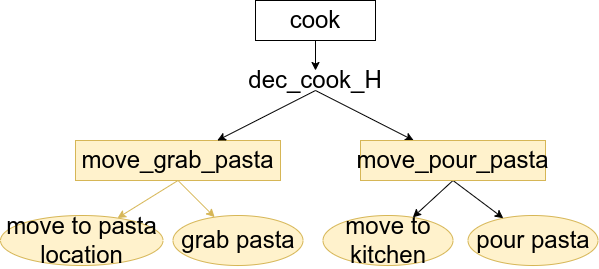
\includegraphics[width=0.4\linewidth]{figures/htn_human.png}
%     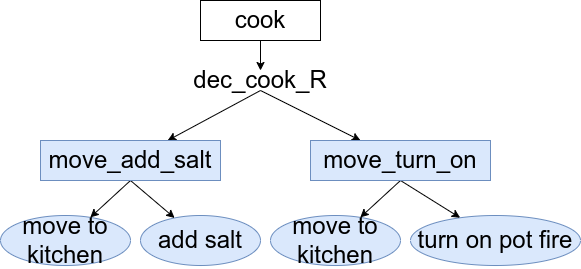
\includegraphics[width=0.4\linewidth]{figures/htn_robot.png}
%     \caption{[OPTINAL, a textual description should be enough to describe such simple task] HTN, cook task description. Additional methods without the move action are not represented corresponding to when the agent is already at the right location.}
%     \label{fig:htn}
% \end{figure*}




% \subsection{Scenarios detailed}

% In this section we focus on the plans obtained with and without our contribution in three different situations. First, both the human and the robot are initially in the kitchen, but the pasta is in the other room, thus the human will have to leave the kitchen. We consider first the case where the robot starts (A) and then when the human starts (B). The third situation includes an initial belief divergence. This time the pasta is already in the kitchen (robot could have brought them before the human arrives) but the human thinks they are still in the other room (C).  

% For each situation (A,B,C), Fig.~\ref{fig:scenarios} depicts the plan computed with (right side) and without (left side) the contribution. The relevant belief updates concerning the salt and stove status are also shown on the figure for both the human and the robot agents.

% 72
% \textbf{Scenario (A):} The plans obtained with and without the contribution are the same, however it's interesting to notice that the human beliefs are not updated in the same way since the human will not observe the "turn on stove" action of the robot. Without the contribution agents are considered "omniscient", so the human instantly knows about the effects of the robot action even without being in the same room. With the contribution, we plan that the human will not observe the robot action thus their beliefs isn't updated. However, we predict that when coming back in the kitchen the human will assess the effects of the robot action and update their beliefs which is far more realistic and leads to more robust plans.

%73
% \textbf{Scenario (B):} This time the human directly leaves the kitchen and will not attend both robot actions which will make the two plans differ. The plan obtained without the contribution is very similar to the (A) one. Before coming back, the human already knew the salt and stove status which isn't very realistic. With the contribution, since we plan that the human will not be in the same place their beliefs isn't updated after the robot actions. We estimate that when coming back to the kitchen the human will assess that the stove is on.
% However, the "salt" state-variable is only inferrable, not observable, thus we predict that the human will not know about the salt even when back in the kitchen. This belief divergence is detected as relevant since it has on influence on the human plan (they might add salt again in the pot). Thus, we decide to insert a communication action to correct the divergence and remove the ambiguity about the salt.

% 9
% \textbf{Scenario (C):} Now the human thinks the pasta is in the other room, but the robot actually brought it to the kitchen before the human arrives. Without the contribution human next actions are estimated using their beliefs ($\beliefs_\human$) so the human will move to the other room and try to grab the pasta. Since there is no pasta in the other room the grab action will fail with the ground truth (but not with $\beliefs_\human$), which makes the plan not valid. With the contribution, we rely on the fact that the human will update their beliefs themselves by assessing the situation and see that the pasta is already in the kitchen. Thus, no communication is needed to fix the belief divergence.

% \subsection{Quantitative results}

% Let's consider two planning problems. The first one is the pasta cooking problem already introduced. The second one consists in preparing three boxes collaboratively. To be ready a box needs to be filled with a defined number of balls and to have a sticker. When ready a box needs to be sent. Only the human can send boxes and only the robot can apply stickers. Both agents can fill the boxes by picking balls from a bucket, but it can run out of balls. To prevent such case, when there is only one ball left, the human first moves to another room to grab more balls and then comes back to refill the bucket. Stickers are observable but the number of ball inside a box is only inferrable.
% Therefore, belief divergences can occur by filling the boxes while the human is away. In both problem the human can miss observable and inferrable effects of robot actions. 

% We ran the planner, with and without the contribution, on both problems. 
% For each problem we generated a total of 512 different initial states including 448 states (87.5\%) with initial belies divergence, and 64 states where both agent beliefs are initially aligned.

% All results obtained are shown in the table \ref{tab:q_results}. 
% The success rate (S) is shown in both cases. With the contribution the ratio of successful plans including a communication action is shown (Com). Without the contribution a planning failure can occur in two cases. First, an action may not applicable (NA) with the other agent's beliefs.
% Indeed, if a human action isn't applicable with the robot's beliefs it means the action isn't applicable in reality. On the other hand, a robot action not applicable with the human's beliefs may damage the human trust towards the robot. For instance, the human thinks there is already some salt in the pot and they see the robot adding salt ``again".
% Then, an inactivity deadlock (IDL) can be reached, i.e. if there is a succession of at least four WAIT or IDLE actions. 
% Such deadlocks may occur when the human has a belief divergence making them wait for a robot action which will never occur (H waiting for R to add salt although there is already salt).
% The ratio of failed planning due to non-applicable human action and due to inactivity deadlocks are given in the table as well.

% **Since the existing system do not handle belief divergences at planning level there was no need to check if an action is applicable with other's beliefs. Also, since there was no belief divergences, if an IDL is reached it means that the task specification is broken. But now, IDL can occur due to div**


% **With the contribution belief divergences can occur during the plan taking into account observability. Since without the contribution observability isn't considered agents are considered omniscient which can create ambiguities in scenarios where observability matters.**

% With the contribution the planner always find a valid plan and, in average, about 62\% of them includes a communication action. Considering that 87.5\% of the scenarios includes an initial belief divergence, we note that the robot doesn't communicate systematically and that the estimated situation assessment solves a relevant part of the divergences.

% Without the contribution, when there are no initial belief divergence, the planner always finds a valid plan. However, the plan generated will always consider the agents as omniscient which may lead to ambiguities when executing the plan in real life. Most of the scenarios that include belief divergence induce actions not applicable in other agent's belief (NA) which explains the 21.8\% success rate in average.

% \begin{itemize}
%     \item w/o always working when there is no belief divergence initially. However, the plan generated will always the agents as omniscient which may later lead to ambiguities when executing the plan in real life. 
%     \item belief divergence on pasta location, R:at\_pasta=room H:at\_pasta=kitchen. Without: H try to grab pasta in kitchen but action not applicable in reality. With: Robot com to warn H that pasta are in room. Actually, H will be able to see that the pasta are not in the kitchen, they cannot see where it is but at least it's not in the kitchen, where they thought it was. We currently not handle explicit assessing of not knowing (assessing that the pasta are not here). However our planner still handles the cases because this divergence (here ambiguity) will affect the human plan thus it is considered as relevant, as a consequence R will communication to align $\beliefs_\human$ and remove the ambiguity.
%     \item div on pasta loc always leads to failure without (not app)
%     \item div on pot fire leads to failure (not applicable reality) only if there is no div on pasta loc (otherwise fails before due to pasta div) and if human tries to pour pasta before robot actually turns on fire. If R turn on fire before, it's not applicable with $\beliefs_\human$ but fixes the div.
%     \item failure inactivity deadlock without if H div on pot\_fire or salt = false although it's already done, thus the robot will never do them again and deadlock occurs
% \end{itemize}



% \section{Discussion}
% how do the results fill the gap ?

% Point out ambiguities (created both by the lack of situation assessment and belief alignment) in the plans without contribution. Then, explain how we removed them. 

% The old solver doesn't consider observability. Such hypothesis may lead to ambiguous situations when trying to execute the produced plan, especially when the plan includes non observed actions. This is shown in case (B) of the cooking domain depicted in fig.~\ref{fig:scenarios} where the presence of salt in the pot should be ambiguous for the human. 
% Our approach proposes a far more realistic way to estimate the human beliefs thanks to the situation assessment as presented in the \textit{Qualitative Results}. Also, by reasoning explicitly on the human beliefs our approach is able to detect and prevent those ambiguous situations while avoiding verbosity as shown in the \textit{Quantitative results}. 
% Since what we consider today as a planning failure is in fact a plan with great risk to not be expected, we can say that our approach is much more consistent and produces more robust plans.

% It is relevant to note that the situation assessment mechanism provided with our approach can only assess observable facts and not refute them. If a human wrongly thinks that there is an object $o_1$ in a place $p_1$, when entering that place the human should be able to assess that the object isn't actually in $p_1$. However, despite this lack, our approach still handles such situations since the divergence will be detected as relevant and the human will be communicated to remove the ambiguity. 

% \subsection{Interesting case}

% An interesting case to focus on is a scenario close to (C) with a belief divergence on the pasta location. Both agents are in the kitchen and the pasta is in the other room, but the human thinks the pasta is in the kitchen. Without the contribution we estimate that the human will try to grab pasta in the kitchen which will fails in real life. In reality the human will be able to assess that the pasta isn't in the kitchen and the human will have an ambiguity on the pasta location. The situation assessment mechanism that we provide do not handle such reasoning, it can only assess facts, not refute them. Despite this lack, our contribution still handles that scenario. Indeed, the SA will not update the human beliefs but a relevant belief divergence is detected. Thus, the robot communicates to remove the ambiguity and inform the human about the pasta location.  

% \section{Conclusion}
% what does this mean for us going forward ?

% FUTURE WORK:
% \begin{itemize}
%     \item A more elaborated formula for observability than co-presence. Using geometrical reasoning with a physic simulator.
%     \item Use an entity-based world description to be able to automatically update the $\loc{\fluent{\worldstate}{}{}{}}$.
%     \item A more complex reasoning to decide where to insert the communication action in the plan.
%     \item Enhanced the situation assessment to be able to refute some facts.
% \end{itemize}

\bibliography{bib.bib}

\end{document}
